\chapter{Линейные операторы}



\section{Определитель}

Есть ли какая-нибудь численная характеристика, которая позволяет сказать, что матрица $A\in M_n(K)$ обратима? Для этого вспомним, что обратимость матрицы $A$ равносильна линейной независимости её столбцов. Если эти столбцы представить себе как вектора в пространстве $\mb R^n$, например, при $n=3$ в обычном трёхмерном пространстве, то видно, что вектора линейно независимы тогда и только тогда, когда объём параллелепипеда на них натянутого отличен от нуля. Конечно, в случае пространства, размерности больше трёх понятие параллелепипеда нужно уточнить:

\dfn Пусть $V$ -- векторное пространство размерности $n$ над $\mb R$, тогда для набора  $v_1,\dots,v_n \in V$ определим параллелепипед
$$D(v_1,\dots,v_n)=\left\{\sum_{i=1}^n \lambda_i v_i\,|\, \text{ где } \lambda_i\in [0,1]\right\}.$$
\edfn


Обозначим для краткости $\Vol(v_1,\dots,v_n)= \Vol (D(v_1,\dots,v_n))$. 

Попробуем понять есть ли возможность как-то аксиоматизировать понятие объёма параллелепипеда на пространстве $V=\mb R^n$, так, чтобы его можно было перенести на произвольное пространство над каким угодно полем. Мне будет удобно набор из $n$  столбцов из $\mb R^n$ объединять в матрицу. Итак, отображение объёма $\Vol M_n(\mb R) \to \mb R$ должно удовлетворять следующим свойствам:
\enm 
\setcounter{enumi}{-1}
\item Объём единичного кубика, единичен. То есть $\Vol(E_n)=1$.
\item При растяжении одного вектора объём меняется пропорционально $\Vol(\dots,\lambda v,\dots)=|\lambda|\Vol(\dots,v,\dots)$.
\item Исходя из принципа Кавальери $\Vol(\dots,v,\dots,u,\dots)=\Vol(\dots,v,\dots,u+\lambda v,\dots)$.
\item Если в наборе есть два одинаковых вектора, то $\Vol(\dots,v, \dots, v,\dots)=0$.
\eenm

Перейдём теперь к ситуации над произвольным полем $K$.
Для общего пространства $V$ условие типа 0) не имеет смысла, так как нет возможности выбрать какой-то канонический базис в $V$. Безусловно, модуль числа в свойстве 1) нет возможности определить над произвольным полем так как  возникают сложности с понятием положительности (особенно в конечных полях). Таким образом, заменой свойства 1) над произвольным полем стоит считать
\enm
\item[1')] $\omega(\dots,\lambda v,\dots)=\lambda \omega(\dots,v,\dots)$.
\eenm
Заметим, что если мы находимся над $\mb R$ и  для отображения $\omega \colon V \times \dots \times V \to \mb R$ выполнено свойство  1'), то для отображения $|\omega|$ выполнены свойства 1). 

Наконец, с алгебраической точки зрения свойство 2) означает независимость относительно элементарных преобразований столбцов матрицы. Это не самое удобное условие. Вместо него мы рассмотрим, как кажется, более сильное свойство
\enm \item[2')] $\omega(\dots,u+v,\dots)=\omega(\dots,u,\dots)+\omega(\dots,v,\dots)$.
\eenm
Действительно из свойства 1'), 2') и 3) следует свойство 2): $$\Vol(\dots,v,\dots,u+\lambda v,\dots)= \Vol(\dots,v,\dots,u,\dots)+\lambda \Vol(\dots,v,\dots,v,\dots)=\Vol(\dots,v,\dots,u,\dots).$$
Свойство 3) имеет смысл всегда и менять его, видимо не следует. Давайте немного покрутимся около этих свойств и посмотрим, что нам даёт их наличие.


\dfn[Общее определение полилинейности] Пусть $U_1,\dots,U_l, V$ -- векторные пространства над полем $K$. Отображение $\omega \colon  U_1\times \dots \times U_l\to V $ называется полилинейным, если
$$\omega(v_1,\dots,v_i+\lambda u_i,\dots, v_l)= \omega(v_1,\dots,v_i,\dots, v_l)+\lambda\omega(v_1,\dots,u_i,\dots, v_l).$$
Множество всех полилинейных отображений будем обозначать как $\Hom_K(U_1,\dots,U_l;V)$. Здесь одновременно зашифрованы свойства типа 1')  и  2').
\edfn


\dfn[Форма]
Полилинейное отображение $\omega \colon  V^l\to K $ называется полилинейной формой степени $l$ на $V$.
\edfn

\rm Вообще, формой принято называть любое отображение из векторного пространства в базовое поле.
\erm


\dfn
Полилинейная форма  $\omega \colon V^l\to K$ на пространстве $V$ над полем $K$ называется:
\enm 
\item антисимметричной или кососимметричной, если $\omega(v_1,\dots,v,\dots,v,\dots, v_l)=0$.
\item симметричной, если $\omega(v_1,\dots,v_i,\dots,v_j,\dots, v_l)=\omega(v_1,\dots,v_j,\dots,v_i,\dots, v_l)$
\eenm
\edfn



Теперь стоит  отметить основные свойства, характерные для полилинейных форм. 

\lm Пусть $V$ -- пространство размерности $n$. Для  полилинейного отображения $\omega \colon V^l \to K $ и любого $e_1,\dots,e_n$ -- базиса $V$  выполнено, что
$$\omega(v_1,\dots,v_l)=\sum_{1\leq i_1,\dots,i_l\leq n}\omega(e_{i_1},\dots,e_{i_l})\prod_{j=1}^l a_{i_j,j}, \text{ где $a_{ij}$ -- это $i$-ая координата вектора $v_j$ в базисе $e$.}$$ 
\elm
\proof По условию $v_j=\sum_{i=1}^n a_{ij}e_i$. Тогда $$\omega(v_1,\dots,v_l)=\sum_{i_1=1}^n a_{i_1,1}\omega(e_{i_1},v_2,\dots,v_l)= \dots = \sum_{1\leq i_1,\dots,i_l\leq n}\omega(e_{i_1},\dots,e_{i_l})\prod_{j=1}^l a_{i_j,j},$$
\endproof

Предыдущую лемму можно доказать и в более общей форме -- для произвольных полилинейных отображений. Но сейчас нам это не нужно. Посмотрим, какие дополнительные ограничения накладывает условие кососимметричности. 


\lm Пусть $V$ -- пространство размерности $n$. Для  полилинейного отображения $\omega \colon V^l \to K $ выполнено: \\
1) Если $\omega$ кососимметрично, то $\omega(\dots,u,\dots,v,\dots)= -\omega(\dots,v,\dots,u,\dots)$.\\
2) В случае, если $\chr K \neq 2$, то из  заключения пункта 1), следует кососимметричность.\\
3) Если $\omega$ кососимметрична, то для любой перестановки $\sigma \in S_l$ выполнено, что $\omega(v_{\sigma(1)},\dots,v_{\sigma(l)})= \sgn(\sigma) \omega(v_1,\dots,v_n)$.\\
4) В предположении кососимметричности $\omega(\dots,v,\dots,u,\dots)=\omega(\dots,v,\dots,u+\lambda v,\dots)$.\\
5) В предположении кососимметричности и условия $l=n$ для набора векторов $v_1,\dots,v_n$ и базиса $e_1,\dots,e_n$ выполнено
$$\omega(v_1,\dots,v_n)=\omega(e_1,\dots,e_n)\sum_{\sigma \in S_n} \sgn(\sigma)\prod_{j=1}^n a_{\sigma(j),j}=\omega(e_1,\dots,e_n)\sum_{\sigma \in S_n} \sgn(\sigma)\prod_{i=1}^n a_{i,\sigma(i)},$$
где $a_{i,j}$ -- это $i$-ая координата $j$-ого вектора в базисе $e_1,\dots, e_n$.
\proof Докажем первое утверждение. Распишем 
\begin{align*} 
0&=\omega(\dots,u+v,\dots,u+v,\dots)=\\&=\omega(\dots,u,\dots,u,\dots)+\omega(\dots,v,\dots,u,\dots)+\omega(\dots,u,\dots,v,\dots)+\omega(\dots,v,\dots,v,\dots)=\\ &=\omega(\dots,v,\dots,u,\dots)+\omega(\dots,u,\dots,v,\dots),
\end{align*}
что и доказывает утверждение. Для доказательства второго утверждения предположим, что $\chr K\neq 2$. Тогда, переставляя одинаковые вектора в выражении $\omega(\dots,v,\dots,v,\dots)$ получаем
$$\omega(\dots,v,\dots,v,\dots)=-\omega(\dots,v,\dots,v,\dots).$$
То есть $2\omega(\dots,v,\dots,v,\dots)=0$. Осталось поделить на 2. покажем третий пункт. По определению знака перестановки
$$\sgn(\sigma)=(-1)^{k}, \text{ где $k$ -- число транспозиций в разложении $\sigma$}.$$
Откуда получаем, что применить $\sigma$ это тоже самое, что применить $k$ транспозиций, то есть изменить знак $k$ раз, что и требовалось. Докажем пункт 4)
$$\omega(\dots,v,\dots,u+\lambda v,\dots)=\omega(\dots,v,\dots,u,\dots)+\lambda\omega(\dots,v,\dots, v,\dots)=\omega(\dots,v,\dots,u,\dots).$$
Для доказательства свойства 5) воспользуемся общим выражением для полилинейной формы из предыдущей леммы
$$\omega(v_1,\dots,v_n)=\sum_{i_1,\dots,i_n} \omega(e_{i_1},\dots,e_{i_n}) \prod_{j=1}^n a_{i_j,j}.$$
Если два индекса совпадают, то $\omega(e_{i_1},\dots,e_{i_n})=0$, а вместе с ним и всё слагаемое. Остаются только наборы с разными $i_{\alpha}$, которые однозначно задают перестановку $\sigma(k)=i_k$. Теперь заметим, что $\omega(e_{\sigma(1)},\dots,e_{\sigma(n)})=\sgn(\sigma)\omega(e_1,\dots,e_n)$, что доказывает первое равенство. Теперь
$$\prod_{j=1}^n a_{\sigma(j),j}=\prod_{i=1}^n a_{i,\sigma^{-1}(i)}.$$
Если вместо $\sigma$ поставить сумму по $\sigma^{-1}$, то с одной стороны сумма не поменяется, а с другой стороны по тождеству выше, можно будет перекинуть $\sigma$ на другой индекс.
\endproof
\elm







\dfn
Пусть $n=\dim V$. Антисимметричная полилинейная форма $\omega \colon V^n \to K $ называется формой объёма на $V$. Если такая форма не равна 0, то будем говорить, что она невырождена.
\edfn



До этого момента мы говорили про объекты которых, возможно, просто не существует. Настала пора предъявить для них конструкцию и доказать её единственность. Для этого достаточно заметить, что все формы объёма, если их расписать в координатах пропорциональны фиксированной функции от координат векторов. Дадим название этой функции:

\dfn  Определителем $\det$ называется отображение $\det \colon M_n(K) \to K$, такое, что $$\det(A)=\sum_{\sigma \in S_n} \sgn(\sigma)\prod_{1\leq i\leq n} a_{i\sigma(i)}.$$
\edfn

Используя понятие определителя можно попытаться определить форму объёма, связанную с фиксированным базисом. Значение получившегося отображения на  самом исходном базисе (с учётом порядка) будет равно единице.

\dfn Пусть $e_1,\dots,e_n$ базис пространства $V$. Определим отображение $\Vol_e \colon V^n \to K$, такое, что
$$\Vol_e(v_1,\dots,v_n)=\det(e(v_1),\dots, e(v_n)),$$
где $e\colon V \to K^n$ -- отображение сопоставления координат.
\edfn

\thrm Верны следующие свойства:\\
1) Определитель является формой объёма на $K^n$, такой, что $\det E=1$.\\
2) Если $V$ -- пространство размерности $n$, то любая форма объёма на $V$ имеет вид $$\omega=\omega(e_1,\dots,e_n)\Vol_e.$$
В частности, если есть два базиса $e$ и $f$, то $\Vol_{f}=\det(C_{f \to e}) \Vol_{e}$.\\
3) Пространство форм объёма одномерно.\\
4) Для любой невырожденной формы объёма $\omega$ верно утверждение: $\omega(v_1,\dots,v_n)=0$ тогда и только тогда, когда $v_1,\dots,v_n$ линейно зависимы.
\proof Определитель является полилинейной функцией столбцов, так как  каждое слагаемое содержит ровно одну координату в первой степени из каждого столбца матрицы $A$. Осталось показать, что если в матрице $A$ пара столбцов одинакова, то её определитель равен нулю.
Пусть равны столбцы $k$ и $l$. Рассмотрим транспозицию $\tau=(kl)$. Тогда все перестановки разбиваются на классы $A_n$ и $\tau A_n$. Выпишем теперь сумму
$$\sum_{\sigma \in S_n} \sgn(\sigma)\prod_{j=1}^n a_{j\sigma(j)} = \sum_{\sigma \in A_n} \prod_{j=1}^n a_{j\sigma(j)}- \sum_{\tau\sigma \in \tau A_n}\,\,\, \prod_{j=1}^n a_{j\tau(\sigma(j))}.$$
Посмотрим на слагаемое в первой и во второй сумме, соответствующие одной и той же перестановке $\sigma \in A_n$. Заметим, что $a_{j\tau(\sigma(j))}=a_{j\sigma(j)}$, если $\sigma(j)\neq k,l$. Но при  $\sigma(j)=k,l$, благодаря тому что $\tau$ переставляет $k$ и $l$, а так же равенству столбцов матрицы $A$, имеем $a_{j\tau(\sigma(j))}=a_{j\sigma(j)}$.
Значит, слагаемые для одних и тех же $\sigma$ сокращаются и получается ноль.

Покажем теперь пункт 2. Используя предыдущую лемму, получаем $\omega(v_1,\dots,v_n)=\omega(e_1,\dots,e_n)\Vol_e(v_1,\dots,v_n)$. То есть, форма $\omega$ пропорциональна форме $\Vol_e$ с коэффициентом $\omega(e_1,\dots,e_n)$. Для завершения доказательства осталось вычислить указанный коэффициент пропорциональности между $\Vol_e$ и $\Vol_f$ для базисов $e$ и $f$. Для этого надо вычислить $\Vol_f(e_1,\dots,e_n)$. То есть, надо построить матрицу из координат столбцов $e_i$ в базисе $f$ и посчитать её определитель. Но это матрица перехода $C_{f\to e}$. Итого $\Vol_{f}=\det(C_{f\to e}) \Vol_{e}$. Здесь мы получили, в частности, что любая форма объёма на пространстве $V$  пропорциональна форме $\Vol_e$, что доказывает пункт 3).


Пусть теперь $v_1,\dots,v_n$ набор векторов. Тогда, если $v_1,\dots,v_n$ линейно зависимы, то существует нетривиальная линейная комбинация $\sum \lambda_i v_i=0$. Пусть $\lambda_1\neq 0$, тогда можно считать, что $\lambda_1=1$. Тогда, прибавляя к первому аргументу остальные с соответствующими коэффициентами, получаем набор с нулевым первым вектором. но при таких преобразованиях значение формы объёма не должно меняться. Итого $\omega(v_1,\dots,v_n)=\omega(0,\dots)=0$.
Обратно, если $v_1,\dots,v_n$ независимы, то $\omega=\omega(v_1,\dots,v_n)\Vol_v$. Так как $\omega \neq 0$, то коэффициент пропорциональности $\omega(v_1,\dots,v_n)\neq 0$.
\endproof
\ethrm


Как видно построение форм объёма сводится к построению определителя. Технически, мы всегда будем обращаться с определителями. Поэтому сформулируем важные свойства: 

\lm Для определителей квадратных матриц верны следующие свойства:\\
0) $\det(A)=\det(A^{T})$.\\
1) Определитель не меняется при элементарных преобразованиях первого типа для строк и столбцов. При смене строк местами меняется знак определителя. При домножении строки на $\lambda$, определитель домножается на $\lambda$.\\
2) $\det(AB)=\det(A)\det(B)$.\\
3) $\det \left(\begin{matrix}A & B\\
0 & C \\
\end{matrix}\right)= \det(A)\det(C)$.\\
4) Определитель верхнетреугольных или нижнетреугольных матрицы равен произведению диагональных элементов.\\
5) $\det (A^{-1})=(\det A)^{-1}.$\\
6) $\det \colon \GL(V) \to K^*$
является гомоморфизмом групп.
\proof Свойство 0) мы уже доказали. Из него сразу же следует свойство 1). Докажем 2).\\
Заметим, что форма $B \to \det AB$ линейна по столбцам $B$. Тогда это форма объёма и следовательно она пропорциональна форме $B \to\det B$. Для того, чтобы найти коэффициент пропорциональности, подставим $B=E_n$. Имеем $\det AE_n=\det A= c \det E_n=c$. Откуда для любого $B$ получаем
$$\det AB=\det A \det B.$$\\
Покажем 3). Сначала посчитаем $$\det \pmat E_n& B\\
0& E_m\epmat.$$
Заметим, что с помощью элементарных преобразований 1-го типа из неё можно сделать $E_{n+m}$. Тогда определитель равен 1.
Теперь заметим, что форма $$A \to \det \pmat A & B\\ 0& E_m\epmat $$ форма объёма на $K^n$. Как и раньше подставив $A=E_n$ получаем что коэффициент пропорциональности с $A \to \det A$ равен 1.\\
Теперь отображение $$C \to \det \pmat A& B\\ 0 & C \epmat $$  есть форма объёма, по строчкам $C$. Подставляя $B=E_m$ находим коэффициент пропорциональности $\det A$, что и даёт
$$\det \pmat A&B\\ 0&C \epmat = \det A \det C.$$
 Применяя предыдущее условие несколько раз приходим к пункту 4).\\
Беря равенство $AA^{-1}=E_n $ и считая определитель получаем $\det A \det A^{-1}=E_n$, что завершает доказательство 5). Пункт 6) следует из 2) и того факта, что определитель обратимой матрицы обязан быть обратимым.
\endproof
\elm



С вычислительной точки зрения формула для определителя бесполезна -- в ней $n!$ слагаемых. Но она даёт некоторые важные следствия. Например, то, что определитель есть однородный многочлен степени $n$ с целыми коэффициентами от элементов матрицы (следовательно, понятие определителя можно ввести над любым коммутативным кольцом по этой формуле).

Обычно, для вычисления определителя матрицу приводят элементарными преобразованиями к ступенчатому виду. При таких преобразованиях не сложно проконтролировать, как определитель меняется. В ступенчатом же виде определитель так же легко сосчитать. Посмотрим на конкретные примеры вычисления определителей.



\exm
\enm 
\item Определитель  $\det \left(\begin{smallmatrix} a&b \\ c& d\end{smallmatrix}\right)=ad-bc$.
\item Определитель матрицы $3\times 3$ тоже можно выписать. 
\item Приведём пример, вычислив определитель Вандермонда.
$$\det \pmat 1 & \dots & 1\\
\lambda_1 & \dots & \lambda_n\\
\vdots &&\vdots\\
\lambda_1^{n-1}& \dots & \lambda_n^{n-1} \epmat= \prod_{i>j}(\lambda_i-\lambda_j).$$
Мы не будем слепо следовать методу Гаусса, а используем элементарные преобразования в другом порядке. Сначала вычтем из $n$-ой строки $n-1$-ую с коэффициентом $\lambda_1$. Потом из $n-1$-ой $n-2$-ую и т.д. Получим:
$$\det \pmat 1 & 1& \dots & 1\\
0 & \lambda_2-\lambda_1 & \dots & \lambda_n-\lambda_1\\
\vdots& \vdots &&\vdots\\
0& \lambda_2^{n-2}(\lambda_2-\lambda_1)& \dots & \lambda_n^{n-2}(\lambda_n-\lambda_1) \epmat= \prod_{i>1}(\lambda_i-\lambda_1)\det \pmat 1 & \dots & 1\\
\lambda_2 & \dots & \lambda_n\\
\vdots &&\vdots\\
\lambda_2^{n-2}& \dots & \lambda_n^{n-2} \epmat.$$
\eenm

Мы стартовали с понятия объёма параллелепипеда в $\mb R^n$. Отображение $A \to |\det A|$ удовлетворяет всем предполагаемым свойствам объёма. Может ли тем не менее, определить дать другое определение объёма параллелепипеда, которое даёт отличные от определителя результаты? \\
Оказывается, что нет. И для этого не нужно требовать все свойства объёма. Достаточно знать, что модуль определителя и объём одинаково изменяются при элементарных преобразованиях. Точнее:

\utv Пусть дано отображение $\Volume \colon M_n(\mb R) \to \mb R $, обладающее некоторыми свойствами объёма параллелепипеда: \\
1) $\Volume(E_n)=1$\\
2) $\Volume(\dots,u+\lambda v,\dots,v,\dots)=\Volume(\dots,u,\dots,v,\dots)$\\
3) $\Volume(\dots,\lambda v,\dots)=|\lambda|\Volume(\dots,v,\dots)$\\
Тогда $\Volume(A)=|\det A|$.
\proof Покажем, что эти свойства однозначно позволяют вычислить $\Volume(A)$. Так как отображение $A\to |\det A|$ тоже им удовлетворяет, то это гарантирует их совпадение.  Действительно, если матрицы $A$ вырождена, то элементарными преобразованиями первого типа можно сделать так, чтобы один столбец $A$ стал нулевым. По третьему свойству $$\Volume(v_1,\dots,0,\dots,v_n)=\Volume(v_1,\dots,0\cdot 0,\dots,v_n)=0\cdot \Volume(v_1,\dots,0,\dots,v_n)=0.$$
Если же $A$ невырождена, то элементарными преобразованиями первого типа её можно привести к диагональному виду не меняя определителя. Теперь вынося по свойству 3) диагональные элементы приводим матрицу $A$ к единичному виду. Осталось воспользоваться свойством 1).
\endproof
\eutv


\subsection{Ориентация}

Настало время отдать долги за школьный курс геометрии и поговорить о важном понятии -- понятии ориентации пространства.  Вспомним, что понятие определителя выросло из аксиоматизации свойств объёма и немного его переросло. А именно, для набора элементов из пространства $\mb R^n$ можно посчитать не только объём параллелепипеда на них натянутого (заведомо неотрицательное число), но ещё и некоторый знак. О смысле этого знака и пойдёт сейчас речь.



\dfn Будем говорить, что два базиса пространства $V$ над $\mb R$ одинаково ориентированы, если матрица перехода между ними имеет положительный определитель.
\edfn

\rm Отношение одинаковой ориентированности есть отношение эквивалентности.
\erm

\dfn Выбор одного из классов эквивалентности базисов вещественного векторного пространства $V$ называется заданием ориентации.
\edfn

\exm
\enm
\item Рассмотрим базисы  плоскости $(0,1),(1,0)$ и $(1,0),(0,1)$.  Они имеют разную ориентацию. Ориентация на $\mb R^n$, заданная стандартным базисом называется стандартной. 
\item Вообще, если один базис плоскости получен из другого при помощи поворота плоскости, то они будут одинаково ориентированы.
\item Аналогично, смена порядка двух базисных векторов приводит к смене ориентации. Растяжение одного вектора на положительную константу  не меняет ориентации, а домножение на отрицательное число -- меняет ориентацию.
\eenm


\utv Пусть есть два базиса $e_1,\dots,e_n$ и $f_1,\dots,f_n$ в пространстве $V$ над $\mb R$. Если они имеют разную ориентацию, то их нельзя продеформировать один в другой (внутри пространства базисов).
\proof Определимся с тем, что доказываем. Прежде всего перейдём к координатам. Можно считать, то $V=\mb R^n$ и множество всех базисов -- это множество обратимых матриц. Надо показать, что не бывает непрерывного отображения $f\colon [0,1] \to \GL_n(\mb R)$, так что $f(0)$ и $f(1)$ по разному ориентированы. 

Действительно, посмотрим на $\det (f(t))$. Пусть при $t=0$ выполнено $\det f(0)>0$,  а при $t=1$ выполнено $\det f(1)<0$. Заметим, что $\det f(t)$ непрерывная функция $[0,1] \to \mb R$. Тогда между $0$ и $1$ у неё есть корень. Но если, $\det f(t)=0$, то $f(t)$ вырождена, чего не может быть, так как по условию $f(t)$ -- обратимая матрица для любого $t$.
\endproof
\eutv

\upr Покажите, наоборот, что любые два одинаково ориентированных базиса можно продеформировать друг в друга.
\eupr

\subsection{Линейные операторы и ориентация}

Особо ценным классом линейных отображений являются отображения пространства в само себя. Я буду называть такие отображения линейными операторами на $V$. Сразу отмечу, что в литературе под словом оператор часто подразумевают линейное отображение между произвольными двумя пространствами. В этой ситуации есть специальное слово, говорящее о том, что речь идёт об отображениях из пространства в себя  -- эндоморфизм пространства. Мы, тем не менее, будем использовать узкое значение слова оператор, имеющее тот же смысл, что и понятие эндоморфизм.

\dfn Пусть $V$ -- пространство. Тогда линейное отображение $L\colon V \to V$ называется (линейным) оператором  на пространстве $V$. Пусть $e_1,\dots, e_n$ базис $V$. Тогда матрицей оператора $L$ в базисе $e$ называется матрица $[L]_e^e$ (базисы с разных концов взяты одинаковыми).
\edfn

Это определение удобно, потому что при фиксированном базисе композиции операторов $L_1\circ L_2$ соответствует произведение их матриц $A_1A_2$ в базисе $e$. В частности, если $A$ матрица $L$ в базисе $e$, то оператору $L^n$ соответствует матрица $A^n$. Если бы базисы были выбраны не согласовано, это было бы неверно. 

\dfn Пусть $L\colon V \to V$ -- линейный оператор. Тогда определим $\det L=\det A$, где $A$ -- матрица оператора в каком-то базисе.
\edfn

Априори неясно, не зависит ли данное определение от выбора базиса. Однако сразу можно заметить, что линейный оператор $L$ обратим тогда и только тогда, когда $\det L \neq 0$. Это даёт уверенность в том, что понятие определителя имеет безкоординатный смысл и, значит, инвариантно, относительно замены базиса. Давайте это покажем:

\utv Определитель корректно определён.
\proof Корректность получается из соображения, что при смене базиса $e\to f$ матрица $A$ заменяется на $C_{f\to e}A C_{f \to e}^{-1}$. Считая определитель получаем
$$\det C_{f\to e}A C_{f \to e}^{-1}= \det C_{f\to e} \det A \det C_{f\to e}^{-1}= \det A.$$
\endproof
\eutv



\dfn Пусть $V$ -- векторное пространство над $\mb R$. Будем говорить, что линейный оператор $L\colon V \to V$ сохраняет ориентацию, если $\det L>0$ и не сохраняет, если $\det L<0$.
\edfn

\lm Сохраняющее ориентацию отображение переводит одинаково ориентированные базисы в одинаково ориентированные.
\proof Пусть $e$ -- базис. Если матрица $L$  в базисе $e$ это $A$, то $A$ -- это то же самое, что матрица перехода от $e$ к $Le$, что и доказывает утверждение. Условие сохранения ориентации говорит, что $\det A > 0$, а значит $e$ и $Le$ одинаково ориентированы.
\endproof
\elm

\exm\\
1) Симметрия относительно прямой в $\mb R^2$ меняет ориентацию.\\
2) Поворот сохраняет ориентацию.\\
3) Центральная симметрия в $\mb R^n$ (домножение на $-1$) меняет или нет ориентацию в зависимости  от чётности $n$.\\





Проинтерпретируем наши результаты с случае $\mb R^n$. Возьмём базис $v_1,\dots,v_n$ и пусть $L$ -- задан матрицей $A$. Пусть $B$ -- это матрица составленная из $v_1,\dots,v_n$. Мы знаем, что $\det AB= \det A \det B$. Это значит, что $\det L= \det A$ есть коэффициент изменения между объёмом параллелепипеда, натянутого на $v_i$ и объёма параллелепипеда, натянутого на $Lv_i$. То есть определитель оператора есть коэффициент изменения объёма любого параллелепипеда под действием $L$. Это причина того, что при многомерной замене координат в интеграле вылезает определитель Якобиана -- то есть линейного приближения к исходному отображению.

Стоит отметить, что это отношение не зависит и от выбора невырожденной формы объёма так как любые две формы объёма пропорциональны.


\dfn Определим группу операторов $\SL(V)=\{ L\colon V \to V \,|\, \det L=1\}$. Если $V$ -- вещественное векторное пространство, то это операторы, которые сохраняют понятие объёма и выбор ориентации пространства. $\SL_n(K)$ называется группа матриц с определителем единица.
\edfn







\subsection{Явные формулы в линейной алгебре}

Ещё одно применение определителя -- это возможность выписать явное решение для многих задач линейной алгебры. Посмотрим, как это проявляется. Для начала взглянем на сам определитель. Заметим, что так как определитель линеен по столбцам, то должно иметь место равенство $\det (\dots,v,\dots)= \sum c_i v_i$,  где $v_i$ -- координат столбца $v$, а $c_i$ -- некоторые на зависящие от столбца $v$ коэффициенты. Мы сейчас найдём эти коэффициенты $c_i$. Для того, чтобы сформулировать ответ нам понадобятся несколько определений.

\dfn Пусть $A \in M_{m\times n}(K)$. Пусть $I\subseteq \{1,\dots,m\}$, а $J\subseteq \{1,\dots n\}$. Подматрицей $A_{I,J}$ будем называть матрицу, составленную из элементов $A$, стоящих в строках с номерами из $I$ и в столбцах с номерами из $J$. Минором порядка $k$ матрицы $A$ называется определитель некоторой квадратной подматрицы $M_{I,J}=\det A_{I,J}$, где $|I|=|J|=k$. Если $A\in M_n(K)$, то алгебраическим дополнением элемента $a_{ij}$ называется $A^{ij}=(-1)^{i+j} M_{\ovl{i},\ovl{j}}$.
\edfn



\lm При разложении по $j$-ому столбцу имеет место формула  $$\det(A)=\sum_{i=1}^n a_{ij} A^{ij}.$$
\proof Прежде всего установим эту формулу в простейшем случае $$A=\pmat 1& *\\
0& A_{\ovl{1},\ovl{1}}\epmat. $$
Это следствие вычисления определителя блочной матрицы. Итак, пусть фиксирован столбец $j$. Как же теперь найти коэффициенты при $a_{ij}$ в разложении? Для этого надо в качестве $j$-го столбца поставить стандартный базисный столбец $e_i$ и посчитать определитель. Сделаем это. Напишем матрицу
$$B= \bordermatrix{
 & &       &  j &      & \cr
 & a_{11} && 0 &  & a_{n1}    \cr
 & \vdots& & \vdots& & \vdots\cr
 i &a_{i1}&\dots & 1 &\dots & a_{in} \cr
 & \vdots& & \vdots& & \vdots\cr
 & a_{1n} &  & 0 &      &a_{nn} } $$
и переставим по циклу столбцы, чтобы $j$-ый столбец стал первым, и $i$-ая строчка стала первой. Такое преобразование изменит знак определителя на $(-1)^{i-1+j-1}=(-1)^{i+j}$. А в правом нижнем блоке будет стоять нужная подматрица $A$.
\endproof
\elm
Это свойство называется разложением  определителя матрицы  по столбцу. Аналогичная формула верна и для разложения по строке.


В прошлом разделе мы научились по некоторой формуле определять обратима матрица или нет. Это полезно в различных задачах с параметром, где метод Гаусса напрямую не применим для вычисления определителя. Можно поставить новый вопрос: а можно ли написать формулу для решения системы линейных уравнений при некоторых ограничениях? Ответ на  этот вопрос дают формулы Крамера.

\thrm[Формула Крамера]
Пусть дана система линейных уравнений $Ax=b$ с квадратной матрицей $A$ над полем $K$. Если матрица $A$ --- обратима, то единственное решение этой системы имеет вид $$x_i=\frac{\Delta_i}{\Delta}, \text{ где } \Delta=\det A, \text{ а } \Delta_i \text{ --- определитель матрицы, полученной из  $A$ заменой $i$-го столбца на столбец $b$}.$$
\proof Пусть $x$ такой, что $Ax=b$. За $v_1,\dots,v_n$ обозначим столбцы $A$. Тогда $b=x_1v_1+\dots+x_nv_n$.  Теперь посчитаем определитель $\Delta_i$. Это определитель матрицы $(v_1,\dots,v_{i-1},b,v_{i+1},\dots,v_n)$. Подставим $b=x_1v_1+\dots+x_nv_n$ и раскроем скобки в определителе, пользуясь его полилинейностью. Останется ровно одно слагаемое с $x_iv_i$. Итого
$$\Delta_i=\det (v_1,\dots,v_{i-1},b,v_{i+1},\dots,v_n)= x_i \det(v_1,\dots,v_{i-1},v_i,v_{i+1},\dots,v_n)=x_i\det A=x_i \Delta.$$
\endproof
\ethrm

Итак мы научились явно решать систему линейных уравнений. Заметим, в свою очередь, что столбец $u_j$ в матрице $A^{-1}$ есть решение уравнения $Au_j=e_j$. Тогда по формуле Крамера
$$(A^{-1})_{ij}=\frac{\det(v_1,\dots,v_{i-1}, e_j,v_{i+1},\dots,v_n)}{\det A}=\frac{A^{ji}}{\det A}.$$
Это приводит нас к определению:

\dfn
Присоединённой матрицей к матрице $A$ называется матрица $(\Adj A)_{ij}= A^{ji}$ где $A^{ij}$ -- алгебраическое дополнение элемента $a_{ij}$.
\edfn

\thrm
Пусть $A\in M_n(K)$. Тогда имеет место соотношение
$$\Adj A \cdot A= A\cdot \Adj A= \det(A)\cdot E.$$
\proof[Первое доказательство] Для определённости будем доказывать $A\cdot \Adj A= \det(A)\cdot E$. Посчитаем диагональные элементы. Они имеют вид $\sum_{k=1}^n a_{ik} A^{ik}=\det A$ по формуле разложения по $i$-ой строке для матрицы $A$. 

Посмотрим теперь на внедиагональный элемент в произведении. Он представим суммой $\sum_{k=1}^n a_{ik}A^{jk}$ при $j\neq i$. Рассмотрим матрицу $A'$, в которой все строки, кроме $j$-ой такие же как в матрице $A$, а на место $j$-ой строки поставлена копия $i$-ой. Понятно, что $\det A'= \sum_{k=1}^n a_{ik}A^{jk}$ по формуле разложения по строке. С другой стороны матрица $A'$ вырождена. Поэтому это $0$.

\proof[Второе доказательство] Заметим, что если матрица $A$ обратима, то это уже у нас в кармане. Что же делать для необратимых $A$?
Оказывается, что вместо того, чтобы пытаться как-то свести к тождеству для всех матриц над тем же полем $K$ проще доказать это тождество над любым кольцом. Точнее, заметим, что это тождество равносильно равенству нулю некоторых целочисленных многочленов от коэффициентов матрицы. Это тождество имеет смысл над любыми кольцами. Тогда, если мы доказали это тождество для кольца $R$ и матрицы $B$, и есть гомоморфизм $\ffi \colon R \to S$, то это тождество верно для матрицы $\ffi(B)$ над $S$.

Рассмотрим кольцо $\mb Z[a_{11}, \dots, a_{nn}]$ многочленов от $n^2$ независимых переменных. Над этим кольцом есть матрица $A$, что $A_{ij}=a_{ij}$. Эта матрица называется общей матрицей (размера $n\times n$). Потому что для любой матрицы $B$ размера $n\times n$ над кольцом $R$ есть гомоморфизм $\ffi \colon \mb Z[a_{11},\dots,a_{nn}]\to R $, что $\ffi(A)=B$. Иными словами в эту матрицу можно подставить любые значения.

Таким образом, достаточно доказать наше тождество для одной матрицы $A$. Для этого вложим кольцо
$$\mb Z[a_{11},\dots,a_{nn}] \to Q(\mb Z[a_{11},\dots,a_{nn}]).$$ Тогда достаточно доказать тождество для матрицы $A$ в $Q(\mb Z[a_{11},\dots,a_{nn}])$. Для этого покажем, что матрица $A$ невырождена. Заметим, что её определитель -- это ненулевой многочлен $$\sum_{\sigma \in S_n} \sgn(\sigma) \prod_{i=1}^n a_{i\sigma(i)} \in Q(\mb Z[a_{11},\dots,a_{nn}]),$$ который мы обычно и называем определителем. Раз определитель $A$ не ноль, то $A$ -- невырожденная матрица над полем $Q(\mb Z[a_{11},\dots,a_{nn}])$ и, следовательно для неё тождество выполнено. Что и требовалось.
\endproof
\ethrm

В этом доказательстве мы пользовались возможностью перейти к полю частных и тем, что общая матрица обратима хотя и не над кольцом $\mb Z[a_{11},\dots,a_{nn}]$, но в его поле частных. Если посмотреть, когда ещё можно провернуть похожее рассуждение, то можно сформулировать принцип: если есть некоторое полиномиальное тождество, верное для всех значений переменных, кроме, возможно, тех, которые задаются нетривиальным полиномиальным уравнением $p(x_1,\dots,x_n)=0$, то это тождество выполнено без исключений. Под словом, нетривиальный здесь подразумевается следующее: есть такой набор координат, для которых $p(x_1,\dots,x_n)\neq 0$. 

\upr Покажите, что над любым кольцом $\det(AB)=\det A \det B$.
\eupr


\section{Алгебры}

{\bf {\color{red} Внимание!!!}} Начиная с этого момента под словом кольцо я буду понимать ассоциативное кольцо с единицей. Коммутативно кольцо или нет теперь придётся уточнять.

Настала пора познакомиться с самой навороченной структуры, которая будет у нас в курсе. Начнём издалека. Если есть два пространства $V_1$ и $V_2$ размерностей $n$ и $m$, то имеет место изоморфизм векторных пространств $\Hom(V_1,V_2)\cong M_{m\times n}(K)$. Ничего лучше не сказать, потому что никаких других структур на этих пространствах в общем случае нет. Однако если $V=V_1=V_2$, то пространство $\Hom(V,V)=\End(V)$, то есть множество линейных операторов на $V$ является ещё и кольцом относительно сложения и композиции.  Структура векторного пространства и кольца связаны (кроме дистрибутивности, см. прошлый семестр) ещё одним соотношением:
$$\forall \lambda \in K \text{ и } L_1, L_2 \in \End(V) \text{ верно, что } (\lambda L_1)\circ L_2= \lambda (L_1 \circ L_2)=L_1 \circ(\lambda L_2).$$


\dfn(Алгебра над полем) Пусть $K$ -- поле. Кольцо $S$ вместе с отображением $K \times S \to S$ называется алгеброй, если \\
1) $\forall r \in K$, $\forall u,v \in S$ $r(uv)=(ru)v=u(rv)$.\\
2) $S$ является  векторным пространством над $K$ относительно указанных операций.
\edfn


\rm По нашему соглашению получается, что алгебры всегда ассоциативные кольца с единицей. Стоит понимать, что это всего лишь соглашение в рамках нашего курса. Общепринятое определение не подразумевает этих свойств. Есть важные примеры алгебр, которые не имеют единицы или неассоциативны. Это алгебры функций с компактным носителем в $\mb R^n$ (нет единицы) и так называемые алгебры Ли (нет ассоциативности и единицы). В нашем курсе они не будут систематически появляться.

Можно определить понятие алгебры над произвольным коммутативным кольцом. Дать аналогичное определение над некоммутативным кольцом затруднительно. Причина в свойстве 1).
\erm

Многие из колец, которые появлялись в курсе были алгебрами над каким-то полем:

\exm
\enm
\setcounter{enumi}{-1}
\item Поле $K$ есть алгебра над собой
\item Если $L$ -- расширение поля $K$, то $L$ является алгеброй над $K$.
\item Например, $\mb C$ -- это алгебра над $\mb R$
\item Кольцо эндоморфизмов $\End_K(V)$ векторного пространства $V$ над полем $K$ является алгеброй над $K$. В частности, кольцо матриц над полем $M_n(K)$ есть алгебра над $K$. Это некоммутативная алгебра над $K$ при $n\geq 2$. 
\item То же можно сказать про кольцо верхнетреугольных(нижнетреугольных) матриц $UT_n(K)$.
\item Кольцо многочленов $K[x_1,\dots,x_n]$ есть алгебра над $K$.
\item Любой фактор кольца многочленов $K[x_1,\dots,x_n]/I$ есть алгебра над $K$.
\item Разберём для разнообразия ещё одну конструкцию, которая приводит к интересным некоммутативным алгебрам. Представим себе векторное пространство $V$ с базисом $e_1,\dots,e_n$. Допустим, хочется завести на $V$ структуру алгебры. То есть необходимо научиться умножать два элемента из $V$. Произвольный элемент из $V$ выглядит как сумма $\lambda_1 e_1+\dots+\lambda_n e_n$. Посмотрим, что должно происходить при перемножении двух таких элементов:
$$(\sum_{i=1}^n \lambda_i e_i)\cdot (\sum_{j=1}^n \mu_j e_j)=\sum_{i,j} \lambda_i\mu_j (e_i\cdot e_j).$$
Таким образом видно, что произведение на самом деле достаточно определить только на базисных элементах, а дальше продолжить на все элементы пользуясь указанной выше формулой. Это гарантированно даст структуру кольца. Однако, нам стоит разобраться, когда такая операция даст ассоциативную кольцо. Оказывается, что для этого достаточно ассоциативности умножения на базисных элементах $(e_i\cdot e_j)\cdot e_k=e_i\cdot (e_j\cdot e_k)$. Действительно
$$\left((\sum_{i=1}^n \lambda_i e_i)\cdot (\sum_{j=1}^n \mu_j e_j)\right)\cdot(\sum_{k=1}^n \nu_k e_k)= \sum_{i,j,k} \lambda_i\mu_j \nu_k (e_i\cdot e_j)\cdot e_k=\sum_{i,j,k} \lambda_i\mu_j \nu_k e_i\cdot (e_j \cdot e_k)=(\sum_{i=1}^n \lambda_i e_i)\cdot \left((\sum_{j=1}^n \mu_j e_j)\cdot(\sum_{k=1}^n \nu_k e_k)\right)$$
Теперь осталось привести конкретный пример: пусть $G$ группа из $n$ элементов (можно конечно и не конечную брать -- к чему это приведёт подумайте сами). Групповой алгеброй $K[G]$ над полем $K$ назовём следующую алгебру: возьмём пространство столбцов размера $n$, занумеруем элементы стандартного базиса элементами группы $G$ (любым способом). Соответствующий $g\in G$ базисный вектор будем обозначать $e_g$. Унаследуем умножение на базисных векторах с элементов группы:
$$e_g e_h=e_{gh}.$$
Это определяет структуру алгебры на $K^n$, которая и называется групповой алгеброй. $K[G]$ некоммутативна тогда и только тогда, когда $G$ некоммутативна. Это центральный объект теории представлений групп -- важной области, использующейся в физике.
\eenm





\dfn Отображение $f \colon S_1 \to S_2$, где $S_1$ и $S_2$ являются $K$-алгебрами, называется гомоморфизмом $K$-алгебр, если $f$ -- гомоморфизм колец и линейное отображение.
\edfn



\rm Алгебра эндоморфизмов $\End_K (V)$  изоморфна,  алгебре матриц $M_{\dim V}(K)$.
\erm

В теории групп любая конечная группа могла быть реализована как подгруппа в $S_n$. Оказывается, что мы давно знаем алгебру, которая играет аналогичную $S_n$ роль.



\thrm[Теорема типа Кэли] Любая алгебра $A$, конечномерная над полем $K$, вкладывается в $\End_K(A)$ (то есть фактически в кольцо матриц).
\proof Пусть $x\in A$. Тогда рассмотрим отображение $L_x \colon A \to A$, заданное по правилу $L_x(z)=xz$. Тогда $L_x\circ L_y=L_{xy}$. Так же $L_x+L_y=L_{x+y}$, а $L_1=\id_A$. Заметим, что, если $x\neq 0$, то $L_x$ не нулевое, потому что $L_x(1)=x\neq 0$. Таким образом отображение $A \to \End_K(A)$ заданное правилом $x\to L_x$ является инъективным гомоморфизмом алгебр над $K$, что и требовалось.
\endproof
\ethrm

\rm[Дополнительно] В частности, $\mb C$ вкладывается в алгебру матриц $M_2(\mb R)$ по правилу $a+bi \to \left( \begin{smallmatrix} a &-b\\ b & a \end{smallmatrix}\right) $. Для любой алгебры указанное вложение позволяет ввести понятие нормы: $norm (y)=\det L_y$ -- численная характеристика для любого элемента алгебры за бесплатно. 
\erm



Нам извести, что, если  два коммутативных кольца $R$ и $S$  связаны гомоморфизмом $f\colon R \to S$, то есть единственный гомоморфизм $R[x] \to S$ переводящий $x$ в заданный элемент $s \in S$, а на константах, совпадающий с $f$. Он имеет вид $p(x) \to f(p)(s)$. Я буду апеллировать к аналогичной конструкции в несколько другой ситуации.

\rm
Пусть $K$ -- поле, $A$ -- алгебра над $K$. Заметим, что для элемента $y \in A$ и многочлена $p(x)=a_0+\dots+a_n x^n\in K[x]$ можно определить элемент $p(y)=a_0+\dots+a_n y^n \in A$. Соответствие $p(x) \to p(y)\in A$ определяет единственный гомоморфизм $K$-алгебр $\ffi \colon K[x]\to A$ такой, что $\ffi(x)= y$.
\erm



\rm[Дополнительно] Однако не всё так просто, если переменных больше. Пусть $a,b$ два элемента алгебры $A$, которые не коммутируют между собой. Тогда не существует гомоморфизма $K[t_1,t_2]$ переводящего $t_1\to a$, и $t_2 \to b$.
\erm

\upr Является ли условие коммутирования необходимым условием для существования гомоморфизма? Каков ответ для $K[x_1,\dots,x_n]$?
\eupr




\utv Для любого элемента $y$ конечномерной алгебры $A$ существует $p(x)\in K[x]$, $p(x)\neq 0$ такой, что $p(y)=0$.
\proof Рассмотрим набор элементов $1,y,\dots, y^{\dim A}$. Они линейно зависимы. Следовательно, их нетривиальная линейная комбинация равна нулю, что и даёт искомое уравнение.
\endproof
\eutv


\dfn Ядро гомоморфизма $K[x] \to A$, переводящего $x \to y$ является идеалом  $Ann_y\leq K[x]$. Его элементы называют аннуляторами для элемента $y$ из $A$. Если этот идеал не 0 (есть нетривиальный многочлен, аннулирующий $y$), то образующую этого идеала (со старшим коэффициентом 1) называют минимальным многочленом для элемента $y\in A$ и обозначают $\mu_y(x)$. По другому, это многочлен минимальной степени со старшим коэффициентом 1, аннулирующий $y$.
\edfn

Мы только что показали, что в конечномерной алгебре у любого элемента есть минимальный многочлен. Получим из этого простое следствие:

\thrm Любой элемент $y$ конечномерной алгебры $A$ над полем $K$ либо обратимым, либо делитель нуля (с любой стороны).
\proof Рассмотрим минимальный многочлен $\mu_y(x)= x^n+ \dots+a_0$. Пусть $a_0$ свободный член $p(y)$. Если $a_0=0$, то $$y(y^{n-1}+
\dots + a_1)=(y^{n-1}+
\dots + a_1)y=0.$$ Благодаря минимальности оба выражения отличны от 0, что показывает, что $y$ делитель нуля с любой стороны. Если же $a_0\neq 0$, то $$y^{-1}=\frac{1}{-a_0}(y^{n-1}+
\dots + a_1).$$ В частности, обратный элемент в конечномерной алгебре всегда есть многочлен от исходного. Одновременно оба условия выполнены быть не могут так как, если $yb=0$ и $y^{-1}y=1$, то $b=y^{-1}yb=0$.
\endproof
\ethrm

\rm В частности, обратная матрица всегда многочлен от исходной.
\erm

\upr Для бесконечномерных алгебр это неверно.
\eupr

\upr Покажите, что если $L$ расширение поля $K$, то минимальный многочлен любого ненулевого элемента $y\in L$ неприводим.
\eupr





\section{Линейные операторы}

Посмотрим более пристально на алгебру матриц, или, в бескоординатной форме -- алгебру операторов. Конструкции, которые относятся к структуре кольца на пространстве матриц уже встречались нам. Это прежде всего возведение матрицы в степень -- с его помощью мы считали количество путей в графе, распределение людей в городах. Вот ещё один пример:

Рассмотрим последовательность $x_{n+2}=x_{n+1}+x_{n}$, $x_0=a,x_1=b$. Как посчитать $x_{1000}=?$. Для того, чтобы воспользоваться рекуррентой, надо сделать 1000 операций. Можно ли меньше? С одной стороны вы знаете ответ -- надо найти характеристический многочлен и посчитать его корни, а потом свести всё к вычислению геометрической прогрессии.  Однако в этом случае для получения точного ответа придётся возиться с  иррациональными корнями. Попробуем сделать по другому. Заменим наше соотношение системой
$$ \begin{cases} x_{n+1}=x_n+y_n \\
y_{n+1}=x_{n}
\end{cases}.$$
Перепишем её в следующем виде
$$ \pmat x_{n+1}\\ y_{n+1}\epmat = A \pmat  x_{n}\\ y_n \epmat, \text{ где } A=\pmat 1& 1\\ 1& 0 \epmat.$$
Тогда  $x_{1000}$ это первая координата столбца $A^{1000} \pmat b\\ a\epmat $. Итого достаточно просто возвести матрицу в 1000 степень. Заметим, что это частный случай общей задачи: имеется последовательность $x_n$ из $K^m$ удовлетворяющая соотношению $x_{n+1}=Ax_n$. Требуется найти её поведение в зависимости от $n$. Например -- дан  набор состояний $s_1,\dots,s_k$ и даны вероятности перехода между состояниями $a_{ij}$ за один шаг. Вопрос: что произойдёт с системой после $n$ шагов?
Или, сводя к произведению матриц: как ведёт себя степень матрицы в зависимости от $n$? Оказывается, что этот вопрос удобнее решать не на языке матриц, а на бескоординатном языке операторов, по той причине, что в этой ситуации выбор подходящих координат остаётся за нами. 


Какие величины, связанные с оператором $L \colon V \to V$ не зависят от системы координат. Все свойства оператора $L$ можно определить по его матрице в каком-нибудь базисе. Заметим, что если есть два базиса $e$ и $f$, то матрицы $A=[L]_e^e$ и $A'=[L]_f^f$ связаны соотношением $A'=CAC^{-1}$ для некоторой обратимой матрицы $C$. Наоборот, если $A=[L]_e^e$  и $A'=CAC^{-1}$, то $A'$  тоже матрица $L$, но в другом базисе.

\upr Докажите это.
\eupr

Получается, что свойства оператора $L$, не зависящие от выбора координат, это такие свойства его матрицы $A$, которые не меняются когда мы $A$ заменяем на $A'=CAC^{-1}$. Это приводит нас к стандартному определению:  



\dfn Две матрицы $A, B \in M_n(K)$ подобны если существует матрица $C \in \GL_n(K)$, что $A=CBC^{-1}$. Матрицы одного оператора в разных базисах подобны.
\edfn

Изучение операторов -- это тоже самое, что изучение матриц с точностью до подобия. Нам будет удобно прыгать между двумя этими языками. Вернёмся к операторам. Попробуем придумать какие-то свойства не зависящие от выбора базиса.



\dfn Пусть $V$ -- пространство с оператором $L$. Пусть $U\leq V$. Тогда $U$ называется инвариантным подпространством, если $L(U) \leq U$.
\edfn

\rm Это условие позволяет сузить оператор $L$ с $V$ на $U$. Наличие или отсутствие инвариантных подпространств какой-нибудь размерности не зависит от выбора системы координат.
\erm

\lm Пусть $U\leq V$ -- подпространство, а $L \colon V \to V$ -- линейный оператор. Тогда $U$ инвариантно относительно $L$ тогда и только тогда, когда в базисе $e_1,\dots,e_k,e_{k+1},\dots,e_n$, где $e_1,\dots,e_k$ базис $U$ матрица оператора имеет блочно диагональный вид
$$\pmat A&B\\
0&C \epmat$$
\proof Образ $L(e_i)$ при $i \leq k$ лежит в $U$ и раскладывается по базису $U$, то есть по первым $k$ векторам. Значит коэффициенты при последних $n-k$ векторах нулевые. Но это и есть коэффициенты в левом нижнем блоке матрицы $A$.
\endproof
\elm




Посмотрим на простейший случай, когда инвариантное пространство одномерно. Пусть оно порождено вектором $v$. Тогда условие инвариантности перепишется как $L(v) = \lambda v$ для некоторого $\lambda \in K$.


\dfn Пусть $V$ -- пространство с оператором $L$. Тогда вектор $0\neq v\in V$ называется собственным вектором с собственным числом $\lambda$ относительно оператора $L$, если $Lv=\lambda v$.
\edfn





\exm \\
1) Рассмотрим пространство  последовательностей и оператор сдвига $S(x)_n= x_{n+1}$. Тогда собственный вектор -- это геометрическая прогрессия.\\
2) Рассмотрим тот же контекст. Тогда несложно увидеть, что подпространство последовательностей, удовлетворяющих линейному рекуррентному соотношению с постоянными коэффициентами является инвариантным относительно оператора сдвига.\\
3) В задаче про поисковую систему нам нужен был вектор $w$, такой что $P_G w=w$. Это собственный вектор $P_G$ с собственным числом $1$.\\
4) Подпространство многочленов степени меньшей или равной $n$ инвариантно относительно оператора дифференцирования.\\
5) Если $p(x)$ многочлен, то $\Ker p(L)$ инвариантно относительно $L$.\\
6) Пусть $v \in V$. Тогда  $V'=\lan v, Lv, L^2v,\dots \ran$ является инвариантным пространством, порождённым $v$. Такое пространство называется циклическим.\\
7) Рассмотрим алгебру $K[x]/p(x)q(x)$. Тогда подпространство многочленов делящихся на $p(x)$ является инвариантным относительно оператора $f(x) \to x f(x)$ домножения на $x$.\\




Как найти собственные векторы и соответствующие им собственные числа? Оказывается, что проще найти сначала собственные числа.

\dfn Определим характеристический многочлен оператора $L$ как $\chi_L(t)=\det(A-tE_n)$, где $A$ -- матрица $L$ в некотором базисе.
\edfn

\lm Характеристический многочлен корректно определён.
\elm
\proof Пусть $A$ матрица оператора $L$ в базисе $e$, $A'$ -- в базисе $f$, а $C$ матрица перехода откуда-то куда-то. Тогда $A'=CAC^{-1}$. Рассмотрим $\chi_A(t)$, как элемент $K(t)$. Тогда $C$ -- тоже матрица над $K(t)$ и
$$\det(A'-tE)=\det(CAC^{-1}-tCC^{-1})=\det(C(A-tE)C^{-1})=\det(C)\det(A-tE)\det C^{-1}=\det(A-tE).$$
Раз эти выражения равны как элементы $K(t)$, то и как элементы $K[t]$.
\endproof

\utv Элемент $\lambda \in K$ является собственным числом оператора $L$ тогда и только тогда, когда $\lambda$ корень $\chi_L(t)$.
\proof $\lambda$ собственное число тогда и только тогда, когда есть ненулевой $v$, что $Lv=\lambda v$ тогда и только тогда, когда $(L-\lambda \id)v=0$ тогда и только тогда, когда матрица этого оператора вырождена тогда и только тогда, когда $\det (A-\lambda E) =0$.
\endproof
\eutv



\subsection{Коэффициенты характеристического многочлена}

Как мы уже заметили, собственные числа оператора $L$ -- это корни характеристического многочлена $\chi_L(t)$. Найдя характеристический многочлен, то есть найдя его коэффициенты, мы, фактически, найдём и собственные числа. А какое значение имеют коэффициенты характеристического многочлена сами по себе? 


Первый вопрос, который мы зададим про характеристический многочлен, следующий: насколько общим $\chi_L(t)$ бывает? Верно ли, что любой многочлен $f(x)\in K[x]$ ($\deg f \geq 1$) может быть реализован с точностью до обратимой константы как характеристический многочлен некоторой матрицы над $K$?

\dfn Пусть $f(x)\in K[x]$ многочлен $\deg f \geq 1$. Тогда сопровождающей матрицей к $f(x)=x^n+a_{n-1}x^{n-1}+\dots+a_0$ называется 
$$ \pmat  &&&&-a_0\\
1&&&&-a_1\\
&1&&&-a_2\\
&&\ddots&&\vdots\\
&&&1&-a_{n-1}\epmat.$$
\edfn

\utv Характеристический многочлен сопровождающей матрицы равен $(-1)^n f(t)$.
\eutv
\proof Рассмотрим матрицу $A-tE$, где $A$ -- сопровождающая матрица:
$$A-tE= \pmat -t&&&&-a_0\\
1&-t&&&-a_1\\
&\ddots&\ddots&&\vdots\\
&&1&-t&-a_{n-2}\\
&&&1&-t-a_{n-1}\epmat.$$
Прибавим последнюю строку к $n-1$-ой с коэффициентом $t$. Имеем:
$$\det A-tE = \det \pmat -t&&&&-a_0\\
1&-t&&&-a_1\\
&\ddots&\ddots&&\vdots\\
&&1&0&-t^2-ta_{n-1}-a_{n-2}\\
&&&1&-t-a_{n-1}\epmat$$
Поступая так и далее мы придём к определителю
$$\det \pmat 0&&&&-f(t)\\
1&0&&&*\\
&\ddots&\ddots&&\vdots\\
&&1&0&*\\
&&&1&*\epmat=(-1)^{n-1}(-f(t))=(-1)^nf(t).$$
\endproof

\upr Найдите в примерах оператор, матрицей которого является данная матрица или её транспонирование.
\eupr



Коэффициенты многочлена $\chi_L(t)$ являются инвариантами оператора $L$. Давайте посмотрим на них чуть внимательнее.
Прежде всего в глаза бросается, что свободный член это $\chi_L(0)=\det L$.
 

\dfn Пусть $A$ -- матрица размера $n$, тогда $$\Tr A=\sum_{i=1}^n a_{ii}.$$ 
След оператора $L$ -- это след его матрицы. Это определение не зависит от выбора базиса.
\edfn

\rm След матрицы $A$ это $(-1)^{n-1}a_{n-1}$, где $\chi_A(t)= \sum a_{i}t^i$. 
\erm

След оператора обладает массой интересных свойств:

\lm След обладает следующими свойствами: \\
1) Пусть $A$ -- квадратная матрица. Тогда $\tr CAC^{-1}= \tr A$ для обратимой матрицы $C$.\\
2) $\tr AB = \tr BA$ для $A\in M_{n\times m}(K)$ и $B\in M_{m\times n}(K)$.\\
3) След равен сумме собственных чисел с учётом кратностей, как корней характеристического многочлена (над любым полем, где характеристический многочлен раскладывается на линейные множители).\\
4) $\tr A= \tr A^{\top}$.\\
5) $\tr( A + \lambda B) = \tr A + \lambda \tr B$.
\elm
\proof
1) следует из того, что характеристический многочлен не зависит от выбора базиса и, следовательно, его коэффициенты. 2) Если расписать, то равенство эквивалентно
$$\sum_{i,k} a_{ik}b_{ki}=\sum_{j,l} b_{jl}a_{lj}.$$
Которое верно, особенно если взять $k=j$ и $i=l$. 3) Многочлен $\chi(t)=\prod (\lambda_i-t)$. Осталось раскрыть скобки. 4),5) ясно. \endproof


\rm Аналогично следу, определитель так же выражается через собственные числа. А именно, он равен произведению собственных чисел с учётом их кратностей, как корней характеристического многочлена.
\erm


\rm Для матриц $2\times 2$ знание определителя и следа равносильно знанию характеристического многочлена. Точнее, имеет место формула $\chi_A(t)=t^2-(\Tr A)\, t + \det A$. Для матриц большего размера есть формула для коэффициентов характеристического многочлена через миноры исходной матрицы.
\erm


Поставим следующий вопрос: насколько простой можно выбрать матрицу оператора $L$? Давайте заметим, что как ни крути, матрица линейного отображения должна хранить информацию о характеристическом многочлене, в частности -- о его корнях. Итого, не менее чем $k=\dim V$ параметров должно остаться. Наше чувство прекрасного или же чувство лени подсказывает нам, что самая удобная форма матрицы  -- это диагональная матрица:
$$\pmat \lambda_1 & 0 &\dots & 0\\
0 & \lambda_2 & &0 \\
\vdots && \ddots &\vdots \\
0 & \dots & 0 & \lambda_k \epmat$$

В таком виде как раз возникает $n$ параметров. С другой стороны такой вид матрицы облегчает её возведение в степень. А именно, степень диагональной матрицы $L^n$ будет равна:
$$\pmat \lambda_1^n & 0& \dots & 0\\
0 & \lambda_2^n & &0 \\
\vdots && \ddots &\vdots \\
0 & \dots & 0 & \lambda_k^n \epmat.$$
Теперь начнём подробный разбор:


\dfn Оператор называется диагонализуемым,  если в некотором базисе $V$ его матрица диагональна. Матрица $A\in M_n(K)$ называется диагонализуемой, если соответствующий оператор $x\to Ax$ диагонализуем. Иными словами, должна существовать обратимая $C\in M_n(K)$, что $CAC^{-1}$ -- диагональна. 
\edfn



\lm Матрица оператора $L$ в базисе $v_1,\dots,v_n$ диагональна тогда и только тогда, когда все $v_i$ -- собственные вектора $L$. В этом случае на диагонали матрицы стоят собственные числа оператора $L$.
\proof Если $Lv_i=\lambda_iv_i$, то в $i$ столбце $\lambda_i$ стоит на диагонали, а остальное -- $0$.
\endproof
\elm



\lm Пусть $v_1,\dots,v_n$ собственные вектора $L$ c собственными числами $\lambda_1,\dots,\lambda_n$. Пусть числа $\lambda_i$ попарно различны. Тогда $v_1,\dots,v_n$ линейно независимы.
\proof Пусть есть нетривиальная линейная комбинация $$\sum c_i v_i=0,$$
состоящая из минимально возможного числа векторов (пусть они нумеруются от 1 до $k$). Это означает, что все $c_i\neq 0$. Тогда, применив отображение $L$ получаем
$$0=L\left(\sum c_i v_i\right)= \sum c_i \lambda_i v_i$$
Умножая на $\lambda_1$ и вычитая получаем $$0=\sum_{i=2}^k c_i(\lambda_1-\lambda_i)v_i$$
Если в последней сумме есть хоть одно ненулевое слагаемое, то приходим к противоречию. но это бывает только если $\lambda_i=\lambda_1$ для всех $i$, что невозможно из условия леммы.
\endproof
\elm

\dfn[Алгебраическая и геометрическая кратность] Пусть $L$ оператор на пространстве $V$. Алгебраической кратностью собственного числа $\lambda$ называется его кратность как корня характеристического многочлена $\chi_L(t)$. Геометрической кратностью $\lambda$ называется размерность $\Ker L-\lambda \id$.
\edfn

\lm Пусть $L$ -- линейный оператор на пространстве $V$, а $\lambda$ -- его собственное число. Тогда алгебраическая кратность $\lambda$ не меньше его геометрической кратности.
\elm
\proof Пусть $k$ -- это геометрическая кратность $\lambda$. Тогда есть $k$ линейно независимых собственных векторов $e_1,\dots,e_k$ с собственным числом $\lambda$. Их можно дополнить до базиса. Полученная матрицы оператора $L$ будет иметь блочный вид, в первом блоке которого будет стоять матрица $\lambda E_{k}$. Следовательно характеристический многочлен делится на $(t-\lambda)^k$. Таким образом, алгебраическая кратность не меньше $k$.
\endproof

\rm Несложно найти матрицу. с разными алгебраической и геометрической кратностями для собственных чисел:
$$\pmat \lambda & 1 \\ 0& \lambda \epmat.$$
Собственное число $\lambda$ имеет алгебраическую кратность $2$, но геометрическую кратность $1$.
\erm



\thrm[Критерий диагонализуемости] Пусть $K$ -- поле. Пусть все корни $\chi_L(t)$ лежат в $K$.  Тогда оператор $L$ диагонализуем в том и только том случае, когда для всякого собственного числа $\lambda$ его алгебраическая кратность равна его геометрической кратности.
\ethrm
\proof Пусть $L$ диагонализуем. Рассмотрим его базис из собственных векторов и диагональную матрицу $L$ в этом базисе. Заметим, что $\dim \Ker L- \lambda \id $ совпадает с количеством  $\lambda$ на диагонали у этой матрицы, что, с другой стороны, равно алгебраической кратности собственного числа $\lambda$.

Обратно. Сумма алгебраических кратностей $k_i$ собственных чисел равна $$\sum k_i=\deg \chi_L(t)=n=\dim V.$$
Вспомним, что по условию $k_i=\dim \Ker L - \lambda_i \id$. По условию для каждого собственного числа $\lambda_i$, можно выбрать $k_i$ линейно независимых собственных векторов $v_{i1},\dots,v_{ik_i}$.  Если объединить эти наборы, то будет ровно $n$ штук векторов. Покажем их линейную независимость.
Рассмотрим их нетривиальную линейную комбинацию $$0=\sum_{\substack{1\leq i \leq s \\ 1\leq j\leq k_i}} c_{ij} v_{ij}.$$
Разобьём эту сумму сгруппировав собственные векторы с одним и тем же собственным числом. Сумма собственных векторов с одним и тем же собственным числом есть либо собственный вектор с этим же числом, либо 0. Если какое-то слагаемое $\sum_{1\leq j \leq k_i}c_{ij} v_{ij}=0$, то по независимости векторов $v_{ij}$ при фиксированном $i$ получаем, что $c_{ij}=0$. Такие слагаемые можно выкинуть из суммы. Если слагаемых не осталось, значит все коэффициенты с самого начала были нулевыми. 

Пусть в сумме по $i$ есть ненулевые слагаемые -- то есть, слагаемые вида $\sum_{1\leq j \leq k_i}c_{ij} v_{ij}$.  Это собственные векторы для различных собственных чисел $\lambda_i$. Значит их сумма не может быть равна нулю по предыдущей лемме.

Так как число векторов $v_{ij}$ равно размерности пространства $V$, то  из линейной независимости следует, что они образуют базис $V$.
\endproof



\crl Пусть $K$ -- алгебраически замкнутое поле. Если характеристический многочлен не имеет кратных корней, то оператор $L$ диагонализуем.
\ecrl
\proof В этом случае алгебраическая кратность совпадает с геометрической, потому что обе они равны~1.
\endproof






\crl \label{gprog}
Пусть дана последовательность $x_n\in \mb C$ удовлетворяющая линейному рекуррентному соотношению 
$$x_{n+k}+a_{k-1}x_{n+k-1}+\dots+a_0x_n=0,$$
где $a_i \in \mb C$. Рассмотрим многочлен $f(t)=t^k+a_{k-1}t^{k-1}+\dots+a_0$. Пусть у $f(t)$ нет кратных корней. Тогда $x_n=c_1 \lambda_1^n+\dots+c_k\lambda_k^n$, где $\lambda_i$-- корни $f(t)$.
\ecrl

\proof  Пусть $V$ -- пространство последовательностей, заданных линейным рекуррентным соотношением $x_{n+k}+a_{k-1}x_{n+k-1}+\dots+a_0x_n=0$. Оно имеет размерность $k$: в качестве базиса можно взять последовательности, которые начинаются с вот таких вот упорядоченных $k$-шек:
$$(0,\dots,1,\dots,0).$$
Посмотрим как на них действует оператор сдвига: последовательность с началом $(0,\dots,1,\dots,0)$, где $1$ стоит на позиции $1\leq i\leq k$ переходит в последовательность с началом $(0,\dots,1,\dots, -a_{i-1})$, где $1$ стоит на позиции $i-1$, либо $1$ вообще нет, если $i=1$.
Таким образом, матрица оператора сдвига имеет вид: 
$$ \pmat 
&1&& \\
&&\ddots&\\
&&&1 \\
-a_0 & -a_1& \dots & -a_{k-1}
\epmat $$
Но это просто транспонированная матрица к присоединённой для многочлена $f(t)$. Её характеристический многочлен равен $(-1)^nf(t)$. Многочлен $f(t)$ не имеет кратных корней.  По критерию диагонализуемости у оператора сдвига есть базис из собственных векторов, с собственными числами $\lambda_i$ -- корнями $f(t)$. Но собственные вектора для оператора сдвига -- это геометрические прогрессии. Значит в $V$ есть базис из геометрических прогрессий и частные этих прогрессий -- это $\lambda_i$.
\endproof

Даже если все корни характеристического многочлена матрицы  лежат в данном поле, это не значит, что матрица диагонализуется: вот простейший пример 
$$\pmat 0&1\\ 0&0 \epmat.$$

Теперь мы так же можем отчасти ответить на самый первый вопрос: если две матрицы (над $\mb C$) имеют одинаковый характеристический многочлен, и у него нет кратных корней, то они подобны: действительно, они обе подобны диагональной матрице, у которой на диагонали стоят собственные числа их характеристического многочлена.

С другой стороны, если кратные собственные числа есть, то ситуация усложняется. Вот две матрицы, имеющие одинаковый характеристический многочлен, но не подобные:
$$\pmat 0&1\\ 0&0 \epmat\,\,\,\,\, \pmat 0&0\\ 0&0 \epmat.$$
Первая недиагонализуема (по критерию), а вторая уже диагональна.


\section{Подготовка}

Прежде чем дать общий ответ на вопрос о том, что может происходить в случае, если оператор не диагонализуется обсудим несколько лемм и конструкций:



\lm Пусть $L$ -- оператор на пространстве $V$, а  многочлен $g(t)=p(t)q(t)$ аннулирует $L$ (то есть $g(L)=0$). Причём $(p(t),q(t))=1$. Тогда подпространство $V$ раскладывается в прямую сумму инвариантных подпространств
$$V = \Ker p(L)\oplus \Ker q(L).$$
\elm
\proof Рассмотрим линейное разложение $1=a(t)p(t)+b(t)q(t)$. Тогда любой вектор $v$  представим в виде
$$v=a(L)p(L)v+ b(L)q(L)v.$$
Тогда $q(L)a(L)p(L)v=0=p(L)b(L)q(L)v$. Следовательно, $V= \Ker p(L)+\Ker q(L)$. Покажем, что ядра пересекаются по нулю. Пусть $v\in \Ker p(L) \cap \Ker q(L)$. Тогда $v=a(L)p(L)v+ b(L)q(L)v=0$.
\endproof

\upr Как мы уже отмечали, если пространство разложилось в сумму двух $V=U_1\oplus U_2$, то есть оператор проекции, который вектору $v=u_1+u_2$ сопоставляет $u_1$ -- его $U_1$ компоненту. Это отображение называется проекцией на $U_1$ вдоль $U_2$.
Где в доказательстве всплыл оператор проектирования на $\Ker p(L)$ вдоль $\Ker q(L)$?
\eupr


Начнём с того, почему разложение пространства в прямую сумму инвариантных так удобно:

\utv Пусть $L$ -- оператор на $V$, пространство $V=U_1\oplus U_2$, где $U_1,U_2$ инвариантны. Если $e_1,\dots,e_k$ и $f_1,\dots,f_l$ -- базисы $U_1$ и $U_2$, то матрица $L$ в базисе $e_1,\dots, f_l$ имеет вид
$$\pmat A_1 & 0 \\ 0 & A_2 \epmat.$$
Угадайте, что это за матрицы $A_1$ и $A_2$.
\eutv




Прекрасно, когда всё пространство раскладывается в прямую сумму двух инвариантных подпространств. Но так тоже не всегда бывает. Вот более общая конструкция. Надеюсь, за ней вы увидите ранее знакомый алгебраический принцип:

\dfn Пусть $U$ -- подпространство в $V$. Определим на факторе $V/U$ структуру векторного пространства следующим $\lambda \ovl{v}=\ovl{\lambda v})$.
\edfn

\upr Проверьте, что это действительно векторное пространство.
\eupr

\upr Как найти базис $V/U$ зная базис $U$ и базис $V$?
\eupr

\upr Рассмотрим пространство $V=\mb R^4$ и в нём подпространства $U=\lan (1,1,1,1)^\top, (2,2,1,1)^\top \ran$. Найдите базис факторпространства.
\eupr


\dfn Пусть $V$ -- пространство с оператором $L$, а $U$ -- инвариантное подпространство. Тогда определим оператор $\ovl{L}$ на $V/U$ следующим образом:
$$\ovl{L}(\ovl{v})=\ovl{L(v)}.$$
\edfn

\rm Разумеется, вычислять многочлен от оператора на факторпространстве можно на представителях. Формально, если $p(x)$ -- многочлен, а $v\in V$, то $p(\ovl{L})\ovl{v}=\ovl{p(L)v}$.
\erm

\rm Мы уже знаем, что инвариантное подпространство приводит к тому, что в подходящем базисе матрица линейного оператора становится блочно-верхнетреугольной и верхний блок -- это матрица сужения оператора. Дадим интерпретацию нижнего правого блока:  Пусть $e_1,\dots,e_n$ базис $V$ и $\lan e_1,\dots,e_k\ran$ -- инвариантное пространство относительно $L$. Если  матрица $L$ в этом базисе имеет вид $$\pmat A& B \\ 0 & C\epmat,$$
то $C$ -- это матрица $\ovl{L}$ в базисе
$\ovl{e_{k+1}},\dots,\ovl{e_n}$.
Следовательно, $$\chi_L(t)=\chi_{L|_{V'}}(t)\cdot \chi_{\ovl{L}}(t).$$
\erm

Итак, если мы нашли инвариантное подпространство $U$ внутри $V$ относительно $L$, то исследование $L$ в некотором смысле сводится к исследованию $L|_U$ на  $U$ и $\ovl{L}$ на $V/U$. Покажем пример, как это работает.


\thrm[Теорема Гамильтона-Кэли] Пусть $L$ -- оператор на $V$. Пусть многочлен $\chi_L(L)$ раскладывается в $K$ на линейные множители. Тогда $\chi_L(L)=0$.
\ethrm
\proof Докажем по индукции. Случай $\dim V=1$ ясен. Шаг. Так как $K$ алгебраически замкнуто, то у характеристического многочлена есть корень $\lambda_1$ и собственный вектор $e_1$. Рассмотрим фактор $V/\lan e_1\ran$. Для него теорема выполнена. Заметим, что $$\chi_L(t)= -(t-\lambda_1)\chi_{\ovl{L}}(t).$$
Пусть $v \in V$. Тогда $\chi_{\ovl{L}}(L)v = ce_1$ так как в факторе этот элемент равен 0. Но тогда
$$\chi_L(L)v= -(L-\lambda_1 E)\chi_{\ovl{L}}(L)v=-(L-\lambda_1 E) ce_1=0$$
\endproof

\upr Избавьтесь от предположения о том, что многочлен раскладывается на линейные множители (используя какой-нибудь  алгебраический трюк).
\eupr


\rm Теорему Гамильтона-Кэли очень легко доказать, когда $L$ -- диагонализуем.
\erm


\section{Жорданова форма}

В этом разделе я буду предполагать, что  поле $K$ алгебраически замкнуто. Ровно те же результаты можно получить, предполагая, что поле $K$ содержит все корни характеристического многочлена рассматриваемого оператора. В этом разделе мы получим полную классификацию операторов над алгебраически замкнутым полем $K$, то есть для каждого оператора мы построим некоторую матрицу -- его каноническую <<модель>> и научимся строить базис, в котором матрица оператора -- это его <<модельная>> матрица.

\dfn
Матрица $k\times k$
$$J_k(\lambda) = \begin{pmatrix}
\lambda& 1&& \\
& \lambda &1& \\
&&\ddots &\ddots& \\
&  && \lambda & 1\\
&  &&& \lambda
\end{pmatrix}
$$
называется жордановой клеткой размера $k$ с собственным числом $\lambda$.
\edfn

\rm Заметим, что для того, чтобы в базисе $e_1,\dots,e_n$ матрица оператора $L$ была жордановой клеткой необходимо и достаточно, чтобы $(L-\lambda E)e_i=e_{i-1}$ для $i\geq 2$ и $(L-\lambda E)e_1=0$. В частности, оператор $L-\lambda E$ должен быть нильпотентным.
\erm







\thrm Пусть $L\colon V \to V$ --- оператор на конечномерном пространстве над алгебраически замкнутым полем $K$.
Тогда существует базис $e_1,\dots, e_n$ в котором матрица $L$ имеет вид
$$A=\begin{pmatrix}
J_{k_1}(\lambda_1) &&&\\
& J_{k_2}(\lambda_2) &&\\
&& \ddots& \\
&&& J_{k_s}(\lambda_s)

\end{pmatrix}.
$$

Более того, такая матрица единственна с точностью до перестановки блоков. Эта матрица называется матрицей оператора в форме Жордана. Базис, в котором матрица оператора имеет такой вид называется жордановым базисом.
\ethrm
\proof

Сначала докажем единственность. Прежде всего, если нам дана матрица в жордановой форме, то мы легко можем вычислить её характеристический многочлен. Он равен $\prod (t-\lambda_i)$ где $\lambda_i$ -- все числа на диагонали, откуда сразу становится ясно, что $\lambda_i$ -- собственные числа $L$. Более того, алгебраическая кратность
$k$ собственного числа $\lambda$ равна сумме размеров клеток с этим собственным числом.

Пусть сами размеры клеток для собственного числа $\lambda$ заданы как набор чисел $h_i$. Имеем
$\sum h_i =k.$
Итак, набору клеток соответствует разбиение числа $k$ в сумму некоторого числа слагаемых. Удобно упорядочить эти слагаемые по возрастанию $h_i\geq h_{i+1}$.

Можно ли как-то лучше визуализировать себе структуру жордановой формы?
Каждому разбиению числа на слагаемые однозначно соответствует картинка:


\begin{figure}[hhh]
\begin{center}
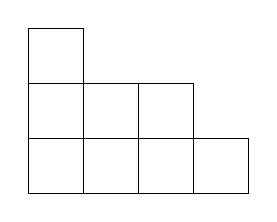
\begin{tikzpicture}[xscale=0.7, yscale=0.7]
\draw (1,0) -- (1,3) -- (0,3) -- (0,0) -- (4,0) -- (4,1) -- (0,1);
\draw (0,2) -- (3,2) -- (3,0);
\draw (2,0) -- (2,2);


\end{tikzpicture}
\end{center}
\caption{$8=3+2+2+1$, соответствует одной клетке размера 3, двум клеткам размера 2, одной клетке размера 1}
\end{figure}

А именно, сопоставим каждому слагаемому $h_i$ столбик высоты $h_i$. Такие (обычно, правда, перевёрнутые) картинки называются диаграммами Юнга.

Как же восстановить эту картинку зная оператор $L$ и собственное число $\lambda$?

Рассмотрим оператор $N=L-\lambda E$. Понятно, что сколько клеток с $\lambda$ было у $L$ в указанном базисе, столько же клеток с с.ч. 0 будет и у $N$ и они будут такого же размера.
Заметим, что жордановы клетки с собственным числом 0 являются нильпотентными матрицами.



Вспомним, что каждой клетке соответствует кусок базиса из векторов вида  $v_i, N v_i, \dots,N^{h_i} v_i$. Заметим, что эти вектора образуют базис пространства $\Ker N^k$. Действительно, $N^k$ обнуляется на векторах $v_i$ и их образах. С другой стороны $N^k$ обратим на дополнительном слагаемом.

Пририсуем эти вектора к нашей картинке следующим образом -- поместим $v_i$ наверху соответствующего клетке  столбика, $N v_i$ на ступень ниже и т.д. Таким образом заполним все ячейки диаграммы. При действии оператора $N$ на диаграмму происходит следующее -- все вектора съезжают на единицу вниз, кроме самых нижних, которые переходят в $0$.
\begin{figure}[hhh]
\begin{center}
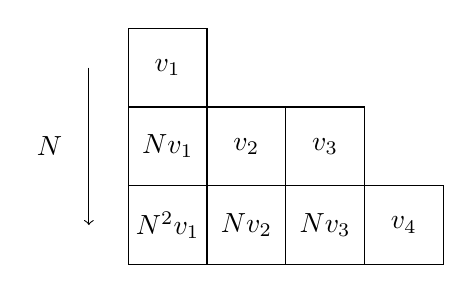
\begin{tikzpicture}[xscale=1, yscale=1]
\draw (1,0) -- (1,3) -- (0,3) -- (0,0) -- (4,0) -- (4,1) -- (0,1);
\draw (0,2) -- (3,2) -- (3,0);
\draw (2,0) -- (2,2);
\draw[->] ( -0.5, 2.5) -- (-0.5, 0.5);
\node at (0.5, 2.5) {$v_1$};
\node at (0.5, 1.5) {$Nv_1$};
\node at (0.5, 0.5) {$N^2 v_1$};
\node at (1.5, 1.5) {$v_2$};
\node at (1.5, 0.5) {$Nv_2$};
\node at (2.5, 1.5) {$v_3$};
\node at (2.5, 0.5) {$Nv_3$};
\node at (3.5, 0.5) {$v_4$};
\node at (-1, 1.5) {$N$};
\end{tikzpicture}
\end{center}
\caption{$8=3+2+2+1$, расставляем базисные вектора}
\end{figure}
Итого, количество ячеек в диаграмме Юнга для собственного числа $\lambda$ оператора $L$ на высоте не более $s$ равно $\dim \Ker(L - \lambda E)^s $.
Это  позволяет однозначно восстановить разбиение числа и, следовательно, конфигурацию клеток, если мы знаем числа $\dim \Ker(L - \lambda E)^s $.

Точнее, число ячеек в строке уровня $s$ равно $\dim \Ker(L - \lambda E)^s -\dim \Ker(L - \lambda E)^{s-1} $.







\proof[Существование]


Для начала надо разбить всё пространство на куски с одним и тем же собственным числом. По теореме Гамильтона-Кэли оператор $L$ аннулируется многочленом $\chi_L(t)$. Разложив последний на простые множители $\chi_L(t)=\prod (x-\lambda_i)^{\alpha_i}$ получим разложение $V=\bigoplus V_i$ на примарные инвариантные подпространства $V_i=\Ker (L-\lambda_i E)^{\alpha_i}$. Ограничимся на пространства $V_i$. Эти пространства называются корневыми. Заметим, что оператор $N=L-\lambda_i E$ нильпотентен. Осталось применить следующую  лемму к операторам $N|_{V_i}$.

\lm[Основная] Для любого нильпотентного оператора $N$ на пространстве $V$ существует базис $e_1,\dots,e_n$ в котором матрица $N$ имеет вид
$$A=\begin{pmatrix}
J_{k_1}(0) &&&\\
& J_{k_2}(0) &&\\
&& \ddots& \\
&&& J_{k_s}(0)
\end{pmatrix}.
$$
\elm
\proof
Докажем по индукции. Если $V=\Ker N$, то матрица просто 0 и всё доказано. Иначе рассмотрим пространство $\Ker N$. Тогда для $V/\Ker N$ теорема верна. Рассмотрим требуемый базис $V/\Ker N$ $\ovl{\ovl{e_{ij}}}$, где первый индекс обозначает номер клетки $1\leq i \leq s$, а второй -- номер вектора(сверху вниз) в  диаграмме Юнга для $V/\Ker N$ -- $0\leq j\leq h_i-1$.
Рассмотрим вектора $e_{i0}$, которые лежат в классе $\ovl{\ovl{e_{i0}}}$ и определим $$e_{ij}=N^{h_i-j}(e_{ih_i}),$$ где  $j\in \ovl{0,h_i}$. Имеет место равенство $$\ovl{e_{ij}}=\ovl{\ovl{e_{ij}}}.$$
Рассмотрим набор векторов $e_{i,h_i}$ -- это вектора из $\Ker N$.
Покажем, что они линейно независимы и, в частности, не 0. Пусть $\sum_{i=1}^s c_ie_{i,h_i}=0$. Это значит $N(\sum_{i=1}^s c_i e_{i,h_i-1} )=0$. Тогда $\sum_{i=1}^s c_i e_{i,h_i-1} $ лежит в ядре $N$. Но в этом случае $\sum c_i \ovl{e_{i,h_i-1}}=0$ в $V/\Ker N$, чего не может быть, так как они там линейно независимы.

Теперь дополним набор $e_{1,h_1},\dots,e_{s,h_s}$ до базиса $\Ker N$  элементами $e_{s+1,0},\dots,e_{k,0}$. Я утверждаю, что  дополненный набор 
$$e_{ij}, \text{ где } 1\leq i\leq k, \,\, 0\leq j\leq h_i (\text{ при } j\leq s) \text{ и } j=0 \text{ иначе }$$
является нужным базисом. Для этого необходимо показать, что он базис. Рассмотрим отображение $V \to V/\Ker N$. Тогда часть этого набора образует базис образа, а оставшаяся часть -- базис ядра. Тогда размерность пространства, порождённого этими векторами равна $\dim \Ker N + \dim V/\Ker N = \dim V$. Откуда получаем, что это базис.

\endproof

\endproof








Допустим мы нашли характеристический многочлен, то есть все его собственные числа. Далее нашли размерности $\dim \Ker(L-\lambda E)^s$. Как теперь найти сам жорданов базис? Для этого нам необходимо заполнить верхушки всех столбцов, остальное заполнится автоматически.



Как расставить векторы в верхней строке диаграммы? Векторы $v_{i_1}, \dots, v_{i_s}$  в верхней строке определяются тем, что их образы при $(L-\lambda E)^{k-1}$ линейно независимы (в частности, не лежат в ядре). Или, (что эквивалентно) система $v_{i_1}, \dots, v_{i_s}$ вместе с базисом (любым) $\Ker (L-\lambda E)^{k-1}$ образуют линейно независимую систему. Напомню, что их число равно
$$s=\dim \Ker (L-\lambda E)^k - \dim \Ker (L-\lambda E)^{k-1}.$$



Что делать с теми клетками, чьи столбики в диаграмме Юнга начинаются не на самом верху? Пусть мы уже заполнили все строки на высоте больше $i$. Заполним остаток строки на высоте $i$.  Очевидно, что оставшиеся векторы лежат в ядре $(L-\lambda E)^{i}$ и при этом их образы при $(L-\lambda E)^{i-1}$ линейно независимы. Однако вектора из уже заполненных клеток на уровне $i$ тоже подходят под это описание. Можно однако заметить, что образы системы <<старые вектора на уровне $i$>>, <<новые вектора на уровне $i$>> при $(L-\lambda E)^{i-1}$ линейно независимы все вместе. Это даёт необходимые условия на оставшиеся вектора в строке $i$.

\lm Выполнено равенство:
$$J_k(\lambda)^n= \pmat \lambda^n & n\lambda^{n-1} & \dots & C_n^{k-1}\lambda^{n-k+1}\\
 &  \lambda^n & &\vdots \\
 &            & \ddots & n\lambda^{n-1}\\
 &&&  \lambda^n \epmat,$$
\elm
\proof Жорданова клетка представима в виде суммы $J_k(\lambda)= \lambda E + N$, где $N$ -- нильпотентная матрица, причём $N^k=0$. На самом деле степени $N$ выглядят следующим образом:
$$N^l= \pmat  & &0& 1& \dots &0 \\
   & && \ddots &\ddots& \vdots\\
 &&&&\ddots& 1\\
 &&&&& 0 \\
 &&&&&  \epmat $$
Теперь
$$(\lambda E+N)^n= \sum_{i=0}^{k-1} C_n^i\lambda^{n-i}N^i,$$
что и даёт требуемое.
\endproof

\crl Пусть $A$ -- матрица из $M_n(K)$. Тогда существует такая обратимая матрица $C$, что $A^n=CJ^nC^{-1}$, где $J$ -- жорданова форма $A$. Причём, матрица $J^n$ составлена из блоков как в предыдущей лемме.
\ecrl
\proof Достаточно взять матрицу $C$ равной матрице перехода из стандартного базиса в жорданов базис для оператора, заданного $A$.
\endproof

\crl Для всякой матрицы $A$ коэффиент её степени $A^n$ есть сумма последовательностей вида $C_n^s\lambda^{n-s}$ с независящими от $n$ коэффициентами. Здесь $\lambda$ -- произвольное собственное число $A$, а $s$ --  меньше, чем максимальный размер жордановой клетки с собственным числом $\lambda$.
\ecrl



\crl Пусть дана последовательность $x_n\in \mb C$ удовлетворяющая линейному рекуррентному соотношению 
$$x_{n+k}+a_{k-1}x_{n+k-1}+\dots+a_0x_n=0,$$
где $a_i \in \mb C$. Рассмотрим многочлен $f(t)=t^k+a_{k-1}t^{k-1}+\dots+a_0$. Тогда $x_n$ есть линейная комбинация последовательностей вида $n^s\lambda^n$, где $\lambda$ -- корень $f(t)$, а $s$ -- строго меньше, чем кратность $\lambda$, как корня $f(t)$.
\ecrl
\proof Как мы помним, матрица оператора сдвига на $V$ -- пространстве последовательностей с заданным линейным рекуррентным соотношением -- имеет характеристический многочлен равный $\pm f(t)$. Пусть $A$ -- матрица оператора сдвига (в стандартном для этого пространства базисе см. следствие \ref{gprog}). Тогда все коэффициенты $A^n$ есть суммы $C_n^s\lambda^{n-s}$.

Если $v$ -- начальный вектор для последовательности, то верхний элемент столбца $A^nv$ равен  $x_n$. Значит последовательность $x_n$ есть сумма последовательностей вида $C_n^s\lambda^{n-s}$ с какими-то коэффициентами. $C_n^s$ -- это многочлен степени $s$ от $n$. Разложив все такие слагаемые в сумму мономов получаем требуемое.
\endproof

\rm[Дополнительно] Последовательностей $C_n^s\lambda^{n-s}$ ровно $k$ штук. Любой элемента $k$-мерного пространства лежит в пространстве, порождённом $C_n^s\lambda^{n-s}$. Значит последовательности $C_n^s\lambda^{n-s}$ лежат в $V$ и являются базисом этого пространства.
\erm

\upr Покажите, что $C_n^s\lambda^{n-s}$ -- это жорданов базис оператора сдвига.
\eupr


\thrm
Пусть $L$ -- оператор на векторном пространстве $V$ над полем характеристики $0$. Тогда матрица оператора $p(L)$ в жордановом базисе $L$ составлена из блоков вида
$$ \pmat p(\lambda) & p'(\lambda) & \dots & \frac{p^{(k-1)}(\lambda)}{(k-1)!}\\
 &  p(\lambda) & &\\
 &            & \ddots & \\
 &&&  p(\lambda) \epmat,$$
где $\lambda_i$ собственные числа, а число и размер блоков c $\lambda_i$ равны числу и размеру блоков в жордановой форме $L$.
\proof Благодаря линейности по многочлену, достаточно проверить равенство только для возведения $L$ в степень. 
\endproof
\ethrm

\crl Пусть $A$ матрица, тогда $p(A)=C p(J) C^{-1}$, где $p(J)$ составлена из блоков как выше, а $C$ составлена из жорданового базиса для $A$.
\proof Если $J$ -- жорданова форма для матрицы $A$, то $A=CJC^{-1}$, где матрица $C$ составлена из собственных векторов $A$.
\endproof
\ecrl

Для дальнейшего нам понадобится понятие аналитической функции. Это понятие из математического анализа.


\dfn Пусть $D\subseteq K$ -- открытый диск с центром в точке $z_0$ радиуса $r>0$ в $K$, где $K$ -- это либо $\mb C$, либо $\mb R$ (то есть круг или интервал). Будем говорить, что функция $f\colon D \to K$ аналитична, если существует последовательность $a_n
\in K$, что $f(z)=a_0+a_1(z-z_0)+\dots+ a_n(z-z_0)^n+\dots$ для любого $ z\in D$. 
\edfn

\exm\\
1) $e^z$ на всём $\mb C$ или на всём $\mb R$\\
2) Да и вообще, любая элементарная функция на любом открытом диске в области определения.

\fct Если $f(z)$ аналитична в $D$, то ряд $a_1+2a_2(z-z_0)+\dots+na_n(z-z_0)^{n-1}+\dots$ сходится в $D$ и равен $f'(z)$. То есть производная существует и аналична в том же диске.
\efct

\dfn Пусть $A$ квадратная матрица над $K=\mb C$ или $\mb R$.  Пусть $f(z)$ -- аналитическая функция в диске $D$, а все собственные числа $A$ так же лежат в $D$. Тогда определим 
$$f(A)=a_0+a_1(A-z_0E)+\dots+a_n(A-z_0E)^n+\dots,$$
относительно покоэффициентной сходимости на $M_n(K)$.
\edfn






\rm  В этом случае матрицу $f(A)$ корректно определена и её можно посчитать следующим образом
$$f(A)= C f(J) C^{-1}.$$
\erm

\rm Особенную популярность функция от матриц получает при решении системы линейных однородных дифференциальных уравнений 
$$x'(t)=Ax(t).$$
Решение даётся в виде $e^{At}C_0$, где $C_0$ -- вектор начальных данных. Это корректно определённое выражение так как ряд для экспоненты сходится везде.
\erm

Есть возможность избежать вычисления самой жордановой формы, обойдясь вычислением характеристического многочлена для того, чтобы посчитать функцию от матрицы. Разберёмся со случаем многочлена от матрицы. 

Допустим мы хотим посчитать $p(A)$, где $p(x)$ -- многочлен c коэффициентами $K$. Рассмотрим $\chi_A(t)$. Допустим нам удалось найти остаток $$p(t)=q(t)\chi_A(t)+r(t).$$
Подставим $A$ и воспользуемся теоремой Гамильтона-Кэли. Тогда
$$p(A)=r(A).$$
Например, для вычисления $A^n$ необходимо знать $x^n \mod \chi_A(t)$. Такой подход может дать сокращение в матричных умножениях, когда $n$ велико. Например, если вы хотите вычислить $n$-ый член последовательности, удовлетворяющей линейному рекуррентному соотношению можно посчитать $r(x)\equiv x^n \mod f(x)$, а потом посчитать начальный член последовательности  $r(L)v$, где $L$ -- оператор сдвига. Вычислить степени оператора сдвига легко -- сдвинуть последовательность несколько раз.


\upr Предложите способ вычисления характеристического многочлена. 
\eupr


\utv Пусть $A$ -- вещественная (или комплексная) матрица с собственным числом $\lambda_1=1$ кратности 1, а все остальные собственные числа $A$ по модулю строго меньше 1. Если вектор $v= \sum c_i e_i$, где $e_i$ жорданов базис, то $$\lim_{n \to \infty}A^nv= c_1 e_1.$$
\eutv

Где мы видели такие матрицы?


\section{Дополнительно: неотрицательные матрицы и теория Перрона-Фробениуса}
\dfn

В каких задачах нам может пригодиться наблюдение про предельный переход? Вспомним старые примеры: для каждого графа $G$ можно построить  несколько  различных матриц, которые кодируют его структуру. Прежде всего это три квадратные матрицы  размера $n\times n$, где $n$ -- это число вершин $G$. 
Первая -- матрица смежности  $A(G)$, которая полностью определяет граф $G$
$$a_{ij}=\begin{cases} 1, \text{ если вершины $i$ и $j$ соединены ребром}\\
0, \text{ иначе }
\end{cases}.$$

Так же нам уже встречалась матрица случайного блуждания  $P(G)$

$$P(G)_{ij}=\begin{cases}
\frac{1}{d_j}, \text{ если есть ребро $j\to i$}\\
1, \text{ если $i=j$ и из вершины $j$ не исходит рёбер} \\
0, \text{ иначе }
\end{cases}.$$
\edfn

Выражение  $P_G^n v$ вычисляет распределение после $n$ шагов случайного блуждания, если начальное распределение было равно $v$. След матрицы $A(G)^n$ считает количество циклов длины $n$ в графе $G$. Кроме того, спектр графа не зависит от порядка вершин графа и значит по нему можно указать, что два графа не изоморфны.

Не остановимся на этом. Это, не единственные примеры, где нужно знать собственные числа матрицы. Вот ещё один: модель Лесли для распределения по возрастам в популяции.

Зададимся следующим вопросом как можно промоделировать эволюцию распределения людей по возрастам? Прежде всего необходимо завести разбиение людей на группы $F_i$ -- одного возраста. $F_i$ можно выбрать, например, группой людей с одинаковым годом рождения. Или $F_i$ может быть группой людей, родившихся в определённое десятилетие. Для каждой  группы мы можем посчитать два параметра: $f_i$ -- ожидаемое количество потомства от члена группы $F_i$ за выбранный временной промежуток; $s_i$ -- процент от общего числа индивидов группы $F_i$ которые выжили за фиксированный промежуток времени и перешли в группу $F_{i+1}$. Пусть $n_1,\dots,n_k$ -- количества индивидов в группах $F_1,\dots,F_k$. Тогда для тех же самых количеств но в следующий промежуток времени имеет место место соотношение:
$$\pmat n_1 \\ \vdots \\ n_k \epmat_{new}=
\pmat f_1 & \dots &f_{k-1} & f_k \\ 
s_1 && &\\
& \ddots & \\
& &s_{k-1} & \epmat \pmat n_1 \\ \vdots \\ n_k \epmat$$
Мы представляем себе, что популяция в целом может расти и убывать. Так же логично предположить, что при стабильных условиях (то есть тогда, когда коэффициенты $f_i$ и $s_i$ не зависят от времени) наблюдается некоторое равновесие. Точнее распределение населения по возрастам должно стабилизироваться. Это означает, что определённый процент популяции составляют старики, определённый процент -- дети и т.д.
Что всё это означает на матричном языке? Прежде всего ясно, что речь идёт о предельном поведении  последовательности векторов $A^n v_0$, где $A$ -- это матрица Лесли, а $v_0$ -- начальное состояние. 
Сделаем несколько предположений про матрицу $A$. Первое предположение -- у матрицы $A$ есть положительное вещественное число $\lambda$, которое больше по модулю всех остальных  собственных чисел (над $\mb C$).  Так же, будем считать, что это собственное число $\lambda$ не кратное (речь об алгебраической кратности) и собственный вектор для этого числа можно выбрать с положительными компонентами.

В этой ситуации оказывается, что $\lambda$ -- это есть скорость роста, а соответствующий ему собственный вектор $e_1$ отвечает за распределение популяции. Точнее, пусть $e_1,\dots,e_k$ -- жорданов базис для $A$, $e_1$ -- тот самый собственный вектор для $\lambda$. Пусть вектор $v_0$ имеет столбец координат $x=(x_1,\dots,x_k)^\top$ относительно базиса $e$. Последнее предположение состоит в том, что $x_1$ -- коэффициент при $e_1$ не равен нулю. Если мы хотим узнать координаты $A^n v_0$ в жордановом базисе, то нужно найти произведение 
$$J^n x= \pmat 
\lambda^n &&&\\
& \lambda_2^n & O(n\lambda_2^n)&\\
&& \ddots \\
&&& \lambda_k^n 
\epmat
\pmat x_1 \\ \vdots \\ x_k\epmat$$
По нашему предположению все остальные $\lambda_i$ по модулю меньше $\lambda$. Тогда видно, что первая координата есть $\lambda^n x_1$, а остальные есть $o(\lambda^n)$. Это означает, что $A^n v_0= x_1 \lambda^n e_1 + o(\lambda^n)$. Значит, за один шаг размер популяции в пределе меняется в $\lambda$ раз, а предельное соотношение координат для $A^n v_0$ такое же, как у вектора $e_1$. Такое отношение существует, потому что компоненты $e_1$ все не равны нулю.


Итого для понимания того, как устроена последовательность $A^nv$, необходимо представлять себе как устроены собственные числа матрицы $A$ и её собственные вектора. В связи с этим возникает несколько вопросов:\\
1) Нас интересует максимальное по модулю собственное число. Хочется, чтобы это число было вещественным и положительным. Когда это выполнено?\\
2) Какова алгебраическая кратность максимального по модулю вещественного собственного числа (если оно есть)?\\
3) Есть ли другие собственные числа, равные по модулю максимальному?\\
4) В указанных задачах хотелось бы, чтобы собственный вектор $v$ для максимального собственного числа был положительным? Всегда ли можно так сделать?

Понятно, что в общем случае ответ на эти четыре вопроса <<нет>> даже в рамках поставленных задач.

\exm
\enm
\item Рассмотрим граф $1 \rightarrow 2$. У матрицы $P(G)$ собственный вектор для собственного числа $1$ имеет нулевую координату.
\item Рассмотрим граф 
\begin{center}
\begin{tikzpicture}
\node (A) at (0,0) {3};
\node (B) at (1,0.5) {1};
\node (C) at (1,-0.5) {2};
\path[->,font=\scriptsize,>=angle 60]
(A) edge (B)
(A) edge (C);
\end{tikzpicture}
\end{center}
У матрицы $P(G)$ есть два собственных вектора $(1,0,0)$ и $(0,1,0)$ с собственным числом 1.
\item Рассмотрим граф $C_n$ -- ориентированный цикл длины $n$. Его спектр -- это корни степени $n$ из единицы.
\eenm



Сейчас мы докажем, что при некоторых предположениях на матрицу $A$ для неё ответы на все четыре вопроса имеют желаемый ответ. Эти предположения не будут выполнены для матриц $A(G)$ и  $P(G)$ непосредственно, однако мы тем не менее сможем извлечь пользу. Что же общего между указанными в наших примерах матрицами?

\dfn Назовём матрицу $A$ положительной (не путать с положительно определённой матрицей квадратичной формы), если все её элементы $A_{ij}$ строго положительны. Будем писать в этом случае $A>0$.
\edfn

\dfn Назовём матрицу  $A$ неотрицательной, если $A_{ij}\geq 0$. Обозначение $A \geq 0$.
\edfn



\dfn В дальнейшем нам будут удобны следующие обозначения: если $A\in M_n(\mb C)$, то $|A|$ -- это матрица составленная из $|a_{ij}|$. Про вещественные матрицы $A$ и $B$ будем говорить, что $A>B$ или $A\geq B$, если $A-B>0$ или $A-B \geq 0$ соответственно.
\edfn



\thrm[Перрон, 1907] Если матрица $A$ положительна, то наибольшее по модулю собственное число $A$ единственное и является вещественным и положительным. Это собственное число не является кратным корнем характеристического многочлена. Собственный вектор для этого собственного числа положителен.
\ethrm
\proof Пусть $\lambda$ -- наибольшее по модулю собственное число и $Ax=\lambda x$. Можно считать, что $|\lambda|=1$ разделив всю матрицу на $|\lambda|$. Тогда покажем, что $A|x|=|x|$.

Прежде всего мы имеем цепочку неравенств $|x|=|Ax|\leq |A||x|=A|x|$, где все неравенства подразумеваются покомпонентными. Обозначим за $z=A|x|$. Это вектор состоящий из положительных координат и рассмотрим вектор $y=z-|x|$. Вектор $y$ неотрицателен. При этом если $y=0$, то мы доказали то, что хотели. Предположим, что есть координата $y_i>0$. Тогда $Ay$ -- положительный вектор, то есть существует такое $\eps>0$, что $Ay>\eps z$. Распишем это неравенство: $Az - z= Az-A|x|> \eps z$ или же $\frac{A}{1+\eps}z>z$. Ввиду положительности правой и левой части мы без сомнений можем применить оператор $\frac{A^n}{(1+\eps)^n}$ к правой и левой части и получить верное неравенство. Итого имеем цепочку 
$$\frac{A^n}{(1+\eps)^n}z>\frac{A^{n-1}}{(1+\eps)^{n-1}}z> \dots > z.$$
Но оператор $\frac{A}{1+\eps}$ имеет собственные числа по модулю меньшие 1 и поэтому, предел левого выражения равен 0. Противоречие!

Итак, в частности, единица собственное число. Покажем теперь, что нет отличных от единицы собственных чисел с модулем $1$. Пусть $\lambda\in \mb C$ собственное число $A$ с $|\lambda|=1$ и $x \in \mb C^n$ -- соответствующий собственный вектор. Тогда $A|x|=|x|=|Ax|$. Заметим, что все координаты $x$ отличны от нуля. Рассмотрим $i$-ую координату. Имеем $\sum A_{ij}|x_j|=x_i=|\sum A_{ij}x_j|$. Посмотрим на это равенство как на равенство между нормой суммы и суммой норм векторов в $\mb C =\mb R^2$. Хорошо известно, что сумма норм больше или равна нормы суммы и равенство достигается тогда и только тогда, когда вектора сонаправлены. Итого все $x_i$ должны быть сонаправлены, но это означает, что $x=e^{i\ffi} |x|$ и следовательно $\lambda=1$. 

Покажем, что единица не кратный корень. Допустим противное. Есть два случая -- либо есть две клетки с собственным числом $1$, либо клетка ровно одна, но при этом размера по крайней мере $2$. Если есть две клетки, то есть два линейно независимых собственных вектора  $x_1$ и $x_2$. Тогда подберём $c$, так что $x_1-cx_2$ имеет нулевую координату. Получаем противоречие, так как $|x_1-cx_2|$ неотрицательный вектор для 1, но при этом с нулевой координатой. Осталось разобрать случай с клеткой размера $k$. В этом случае все коэффициенты матрицы $A^n$ имеют вид $cn^{k-1}+o(n^{k-1})$. При этом $c$ не всегда $0$. Значит некоторые коэффициенты $A^n$ растут при $n\to \infty$. Но тогда некоторые коэффициенты $A^nx_1=x_1$ тоже растут, что очевидно не так.
\endproof

Бывает полезно ещё одно утверждение, которое позволяет установить максимальность собственного числа для заданной неотрицательной матрицы. Оказывается, что для этого достаточно положительности собственного вектора. Нам удобно будет сформулировать и уточнить это соображение не для матрицы $A$, а для матрицы $A^\top$.

\utv Пусть $A\geq 0$, и у матрицы $A^{\top}$ есть положительный собственный вектор для собственного числа $\lambda$. Тогда $\lambda$ -- наибольшее по модулю собственное число $A$. Если у матрицы $A$ есть собственный вектор $y\geq 0$, то $y$ собственный вектор для числа $\lambda$. 
\eutv
\proof Рассмотрим матрицу $A^{\top}$. Пусть $x$ -- положительный  собственный вектор, соответствующий собственному числу $\lambda$. Пусть $\mu$ -- собственное число для собственного вектора $v$. Тогда 
$$\lambda x^{\top}|v|= x^{\top}A|v|\geq x^{\top}|\mu| |v|=|\mu| x^{\top}|v|.$$
Так как $x^{\top}|v| >0$, то $\lambda\geq |\mu|$. Если же, $y=v=|v|$, то имеет место равенство. Так как для неотрицательного вектора $y$ собственное число $\mu$ тоже неотрицательно
\endproof

\dfn Неотрицательная матрица $A\in M_n(\mb R)$ называется стохастической (по столбцам),  если сумма всех коэффициентов в каждом её столбце равна $1$ (иногда дефолтным считается условие на строки). 
\edfn

\rm Такие матрицы встречаются в теории вероятностей, когда речь идёт о марковских цепях -- процессах с дискретным временем в которых последующие события зависят только от текущего положения, а не от того, как вы в него попали.  
\erm

\crl У стохастической матрицы $A$ единица является максимальным по модулю собственным числом.
\ecrl
\proof Вектор $(1,\dots,1)$ является положительным собственным вектором для $A^{\top}$ с собственным числом $1$. Значит у матрицы $A$ есть собственное число $1$ и оно максимальное. 
\endproof


Вообще говоря матрица $P(G)$ имеет довольно много нулевых компонент. И, строго говоря, заключение теоремы Перрона не всегда верно для $P(G)$, как следует из примеров. Как же наша теория может помочь? Для этого мы схитрим и немного поменяем задачу. А именно, рассмотрим матрицу $$P_{\alpha}(G)=(1-\alpha) P(G) + \alpha\tfrac{1}{n}J_n,$$
где $J_n$ -- матрица из одних единиц, а $\alpha \in (0,1)$. Тогда матрицы $P_{\alpha}(G)$ являются положительными. С точки зрения блуждающего пользователя это означает, что у него есть два режима -- первый, в котором он находится с вероятностью $1-\alpha$ -- это режим брожения по ссылкам, а второй режим -- переход на случайную страницу. Для матрицы $P_{\alpha}(G)$ выполнены условия теоремы и поэтому она имеет единственное не кратное максимальное собственное число, равное $1$. Соответствующий собственный вектор можно выбрать положительным.


То, что у $P_{\alpha}(G)$ все собственные числа по модулю меньше единицы означает, что $P_{\alpha}(G)^kv \to cx$, при $k \to \infty$, где $x$ -- положительный вектор с собственным числом равным 1. Это позволяет приближённо найти $x$, что даёт желаемое распределение весов. Практически, для этого можно взять $k\sim \log n$. Количество точных знаков линейно зависит от $k$. Это позволяет заметно сэкономить на вычислениях по сравнению с теоретическим нахождением собственных векторов. Изучая предел $P_{\alpha}(G)$ при $\alpha \to 0$ можно получить информацию и про исходную матрицу.


Можно ли тем не менее что-то сказать в случае неотрицательных матриц? Ответ на этот вопрос дал Фробениус.

\dfn Пусть $A$ -- неотрицательная вещественная матрица размера $n$. Свяжем с матрицей $A$ ориентированный граф $G$ (возможно с петлями). Вершины $G$ есть числа от $1$ до $n$, а ребро между $j\to i$ есть только в том случае, когда коэффициент $A_{ij}\neq 0$. 
\edfn

\dfn Неотрицательная матрица $A$ называется неприводимой, если связанный с ней граф сильно связен.
\edfn

\rm Это равносильно тому, что нельзя так перенумеровать координаты, чтобы в новых координатах матрица $A$ имела блочно-верхнетреугольный вид 
$$\pmat B & C \\ 0 & D \epmat .$$
\erm

\dfn Неотрицательная матрица $A$ называется эргодической или перемешивающей, если существует такая степень $k$, что $A^k>0$. Ещё такие матрицы называют примитивными.
\edfn

\rm Элемент с индексами $i,j$ матрицы $A^k$ не равен нулю только если в графе $G(A)$ есть путь из $j\to i$ длины ровно $k$. В частности, это означает, что эргодическая матрица неприводима. Так  же, понятно, что если матрица $A^k>0$, то это выполнено и для больших степеней.
\erm

На самом деле оба эти понятия ещё более тесно связаны между собой. 

\lm Пусть $A$ -- неотрицательная неприводимая матрица размера $n$. Тогда для любого $\eps>0$  матрица $A+\eps E$ эргодическая.
\elm
\proof Заметим, что  в графе $G(A)$ есть пути $j\to i$ между любыми двумя вершинами. Их длину можно ограничить числом $n-1$. Граф $G(A+\eps E)$ отличается от $G(A)$ только тем, что около каждой его вершины есть петля. Но наличие петель в каждой вершины позволяет из пути длины $k\leq n-1$ сделать путь длины ровно $n-1$. Значит $(A+\eps E)^{n-1}>0$, что и требовалось.
\endproof



\thrm[Фробениус, 1912] Пусть $A$ -- эргодическая матрица. Тогда у $A$ есть единственное максимальное по модулю собственное число  $\lambda$ и оно вещественно и положительно. Кроме того, число $\lambda$ не является кратным для $A$. Числу  $\lambda$ соответствует положительный собственный вектор.
\ethrm
\proof Пусть $\mu\in \mb R_{>0}$ -- наибольшее собственное число для $A^k$, а $v$ -- соответствующий ему собственный вектор. Тогда 
$$\mu Av= A\cdot A^k v= A^k\cdot A v.$$
Откуда получаем, что $Av$ либо $0$, либо собственный вектор $A^k$ с тем же собственным числом $\mu$. Нулём вектор $Av$ быть не может. Тогда нулём был бы и $A^kv=\mu v$. Значит, это собственный вектор для $A^k$ c тем же $\mu$. Значит он пропорционален $v$, то есть $Av=\lambda v$. Так как $v$ вещественный положительный, матрица $A$ неотрицательна, то $\lambda>0$. То есть $v$ -- положительный собственный вектор для собственного числа $\lambda>0$. 

Заметим, что, $\lambda^k=\mu$. Кроме того, если $\lambda_1,\dots,\lambda_n$ -- все собственные числа матрицы $A$, выписанные с учётом кратности, то $\lambda_1^k,\dots,\lambda_n^k$ -- все собственные числа для $A^k$ с учётом кратности. 

В частности, отсюда следует, что у матрицы $A$ не может быть никаких собственных чисел по модулю равных  $\lambda$ и при этом отличных от $\lambda$. Посмотрев на кратности так же можно понять, что $\lambda$ -- не кратное для $A$ число. 
\endproof

\crl Пусть $A$ -- неприводимая матрица. Тогда у $A$ есть вещественное собственное число $\lambda>0$, которое больше или равно всех остальных собственных чисел по модулю. Это собственное   число не кратно. Соответствующий собственный вектор можно выбрать положительным. 
\ecrl
\proof Матрица $A+\eps E$ эргодическая и значит у неё есть положительный собственный вектор $v$, соответствующий собственному числу $\lambda_{\eps}>0$. Тогда $v$ -- собственный вектор матрицы $A$ с собственным числом $\lambda_{\eps}-\eps$. Так как $v$ положительный, а матрица $A$ неотрицательна, то $\lambda_{\eps}-\eps>0$.

Покажем, что $\lambda_{\eps}-\eps$ не зависит от $\eps$. Действительно, если бы у матрицы $A$ было другое вещественное собственное число, большее $\lambda_{\eps} - \eps$ (могло взяться от другого $\eps'$), то это дало бы собственное число матрицы $A+\eps E$, большее $\lambda_{\eps}$, чего не может быть. Обозначим за $\lambda=\lambda_{\eps}-\eps$.   Посмотрим на другое собственное число $\mu$ матрицы $A$. Тогда $\mu+\eps$ -- собственное число матрицы $A+\eps E$. Мы знаем, что $\lambda >|\mu+\eps|$. Это выполнено для всех $\eps$. Значит $\lambda \geq |\mu|$. Завершая доказательство отметим, что если $\lambda$ -- было бы кратным собственным числом для $A$, то $\lambda_{\eps}$ было бы кратным для $A+\eps E$, чего не может быть.
\endproof

\rm Если величины $f_i$ при $1<i\leq k$ и $s_i$ при $1\leq i<k$ в матрице Лесли положительны, то матрица Лесли эргодическая. Если, скажем, все $s_i>0$ и $f_k>0$, то матрица Лесли, по крайней мере, неприводима.

Если граф $G$ сильно связен, то матрица $P_G$ неприводима. А что на языке графов означает эргодичность матрицы $P_G$?
\erm


\upr Покажите, что если $A$ неотрицательная матрица, то у $A$ есть вещественное собственное число $\lambda\geq 0$, которое больше или равно всех остальных собственных чисел по модулю. Для него есть неотрицательный собственный вектор. Как видно из примеров, большего требовать не получится.
\eupr


\section{Дополнительно: модель Леонтьева}
Модель затраты-выпуск Леонтьева. Предположим, что у нас есть несколько типов товаров. Для выпуска каждого товара нужно вложить сколько-то товаров из представленных типов. Например, для производства угля нужна сталь (для стальных инструментов), а для производства стали нужен уголь и сама сталь (в виде инструментов для добычи железной руды). 

Пусть числа $a_{ij}$ характеризуют, сколько нужно взять единиц $j$-го товара для производства товара $i$. Обозначим за $A$ матрицу, составленную из $a_{ij}$. Если $x$ -- это совокупный выпуск всех товаров за фиксированный промежуток времени. Назовём $x$ вектором производств. Пусть $y$ -- это вектор итогового выпуска товаров для внешнего рынка (то, что не нужно для внутреннего производства). Тогда $y$ и $x$ будут связаны уравнением
$$x=y+Ax.$$
Из этого соотношения легко найти $x=(E-A)^{-1}y$. Таким образом, если мы хотим произвести для внешнего рынка $y$ товаров, то для этого совокупно надо произвести $x$ товаров. 

Модель называется продуктивной, если по любому запросу $y\geq 0$ можно предъявить подходящий вектор  производств $x$. При этом вектор $x$ должен быть неотрицательным. 

Продуктивность модели равносильна неотрицательности матрицы $(E-A)^{-1}$. Как можно переформулировать это условие? Заметим, что $\frac{1}{1-x}$ -- аналитическая функция в диске $|z|<1$. Поэтому, если $\lambda$ -- максимальное собственное число $A$ меньше $1$, то $$(E-A)^{-1}=E+A+A^2+\dots +A^n+\dots$$
является неотрицательной матрицей. Если $\lambda=1$, то $E-A$ просто не обратима. Если $\lambda>1$, то $E-A$ может быть необратимой, а может иметь обратную. Покажем, что тем не менее это не приводит к продуктивной модели. Заметим, что у $A$ есть неотрицательный собственный вектор с собственным числом $\lambda$. Но тогда $v$ -- собственный вектор и для $(E-A)^{-1}$ c собственным числом $\frac{1}{1-\lambda}<0$. Но это значит, что матрица $(E-A)^{-1}$ точно не положительная, так как домножив её на $v$ мы получили вектор с отрицательными компонентами.

\section{Дополнительно: метод итераций и оценки на собственные числа}

Как найти приближённо или оценить максимальное по модулю собственное число матрицы. На самом деле, мы уже видели ответ: необходимо возвести матрицу в степень. Точнее: пусть $A$ -- вещественная матрица, которая имеет единственное максимальное по модулю собственное число $\lambda$ (не кратное). Пусть $e_1,\dots,e_n$ -- жорданов базис для $A$, а $e_1$ -- соответствует собственному числу $\lambda$. Рассмотрим случайный вектор $v\in \mb R^n$. С вероятностью $1$ его $e_1$ компонента не $0$. Тогда $A^nv \sim \lambda^n v$. Пусть $x_1(n)$ -- первая компонента $A^nv$. Тогда, если первая компонента у вектора $e_1$ не ноль, то $$\frac{x_1(n)}{x_1(n-1)} \to \lambda.$$
Для оценки скорости сходимости хотелось бы иметь представление об отношении  $\frac{\lambda}{|\lambda_2|}$.

\begin{comment}

Похожая технология применяется, когда необходимо приближённо найти решение системы $x=Ax+b$, где $A$ -- квадратная матрица. Точнее, пусть собственные числа $A$ по модулю меньше $1$. Возьмём случайный вектор $x_0$ и построим последовательность $$x_i=Ax_{i-1}+b.$$
Покажем, что при указанных условия, эта последовательность стремится к решению системы. Прежде всего заметим, что матрица $E-A$ обратима, и, следовательно, система имеет единственное решение. Пусть это решение --- $x'$. Обозначим $h_i=x_i-x'$. Для $h_i$ получается соотношение:
$$x'+h_i=Ax'+Ah_{i-1}+b.$$
Откуда получаем, что $h_i=Ah_{i-1}$. Но тогда $h_i$ стремятся к нулю. Значит $x_i\to x'$.

\end{comment}

Можно ли как-то из теоретических соображений оценить собственные числа матрицы? Оказывается, что такой способ есть. Пусть $A$ -- вещественная или комплексная квадратная матрица. Рассмотрим строки $A$. Зададим элементы $r_i=\sum_{j\neq i} |a_{ij}|$. Рассмотрим множество замкнутых кругов радиуса $r_i$ с центром в $a_{ii}$ на комплексной плоскости. Эти круги называются кругами Гершгорина. 

\utv Все собственные числа матрицы $A$ лежат в объединении кругов Гершгорина. 
\eutv
\proof Пусть $\lambda$ -- собственное число $A$, а $v$ -- соответствующий собственный вектор. Тогда $Av=\lambda v$. Посмотрим на максимальный по модулю элемент $v$ -- $v_i$ и соответствующую ему строчку. Покажем, что $\lambda$ лежит в круге Гершгорина с номером $i$. Имеем $\sum a_{ij}v_j =\lambda v_i$  и, значит, $\sum_{j\neq i} a_{ij}v_j= (\lambda - a_{ii})v_i $. Имеем неравенство $$|\lambda -a_{ii}||v_i| \leq |v_i|\sum_{j\neq i} |a_{ij}|$$
Сокращая на $v_i$ получаем требуемое. 
\endproof

\rm В частности, это рассуждение даёт критерий невырожденности матрицы -- матрица $A$ невырождена, если сумма модулей её внедиагональных элементов каждой строки меньше модуля диагонального элемента. Такие матрицы называются матрицами с диагональным преобладанием
\erm

\rm
Переходя от матрицы к транспонированной можно получить ещё одну оценку, которая получается из рассмотрения столбцов $A$.
\erm


